\subsection{Experiment Details}
\label{app:experiment_details}


%this choice also allows us to more cleanly compare deterministic vs.\ stochastic rounding, since they will always use the same value of $r^*$.

\subsubsection{Details about Uncomppressed Word Embeddings We Used}
We use the Wikipedia 2014 + Gigaword 5 GloVe embeddings available at \url{http://nlp.stanford.edu/data/glove.6B.zip}, and the 300-dimensional fastText embeddings trained on Wikipedia 2017, UMBC webbase corpus and statmt.org news dataset, available at \url{https://s3-us-west-1.amazonaws.com/fasttext-vectors/wiki-news-300d-1M.vec.zip}.
For the GloVe embeddings which we trained, we used full English Wikimedia dump on Dec. 4, 2017 which was pre-processed by a fastText script~\footnote{https://github.com/facebookresearch/fastText/blob/master/get-wikimedia.sh} while keeping the letter cases and digits.
This corpus has 4.5 billion tokens (vocab size of $400k$).


\subsubsection{Empirical Comparison of Compression Methods}

\subsubsection{Dimension vs. Precision Trade-off}

\subsection{Extended Results}
\label{app:experiment_results}
In Figure~\ref{fig:all_sentiment} we present all our sentiment analysis results, for our different embedding types and the different sentiment analysis datasets.
\todo{I commented out large figure}
%\begin{figure}
%	\centering
%	\begin{tabular} {c c c}
%	% MPQA
%	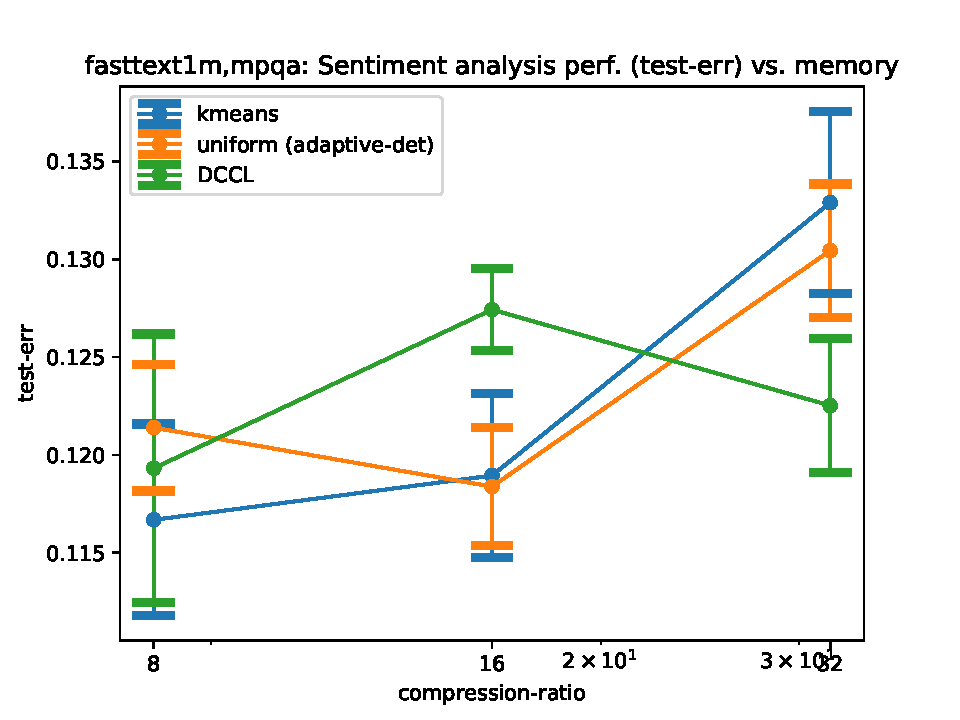
\includegraphics[width=0.28\linewidth]{figures/fasttext1m_mpqa_test-err_vs_compression.pdf} &
%	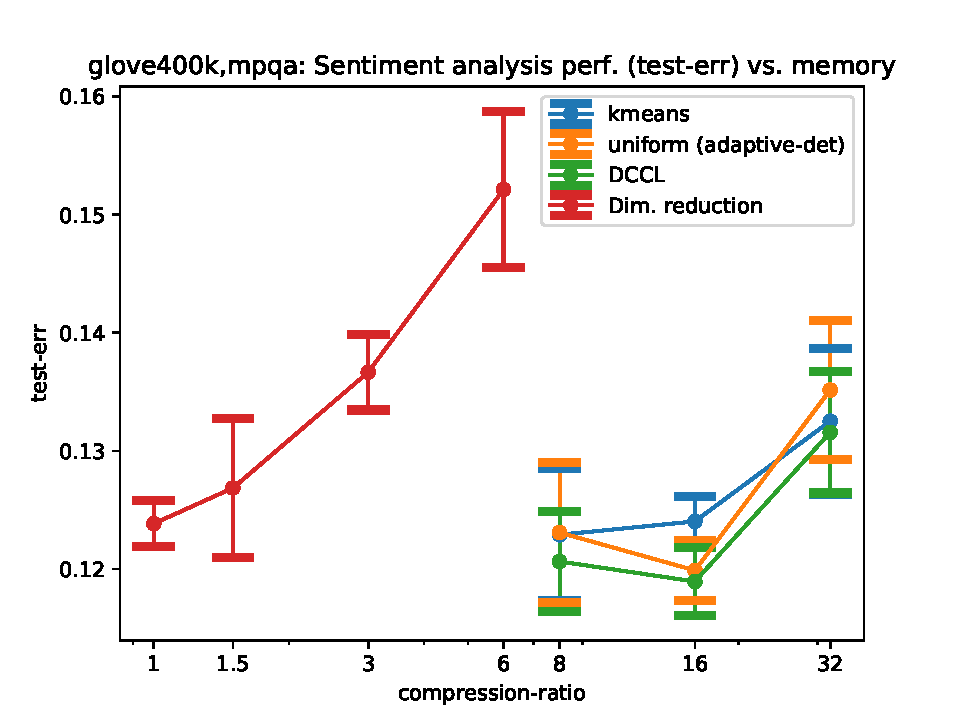
\includegraphics[width=0.28\linewidth]{figures/glove400k_mpqa_test-err_vs_compression.pdf} &
%	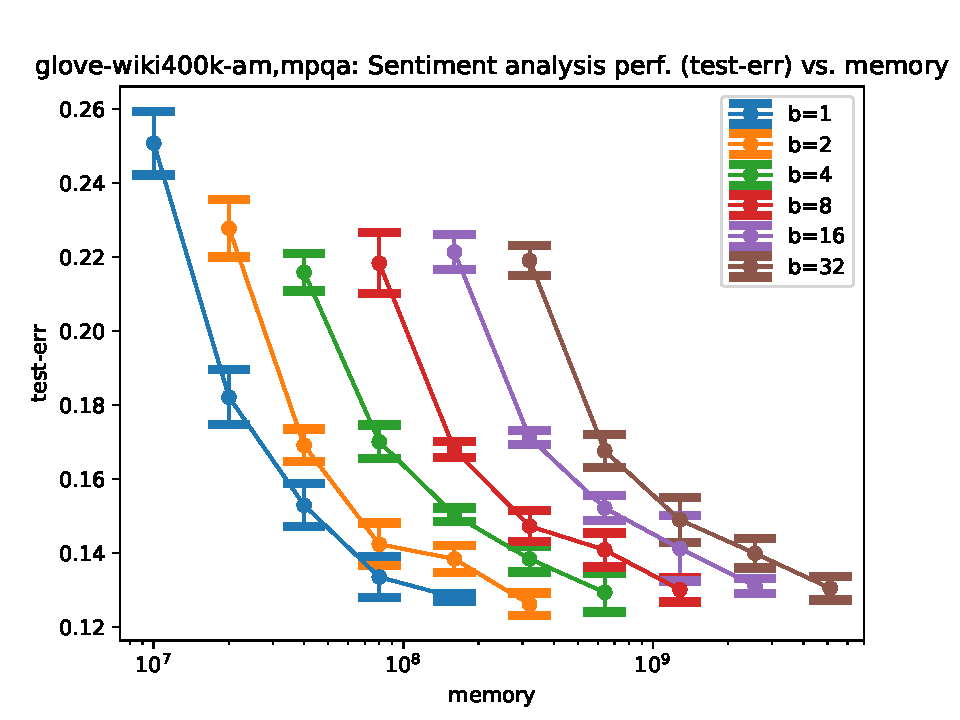
\includegraphics[width=0.28\linewidth]{figures/glove-wiki400k-am_mpqa_test-err_vs_compression.pdf} \\[-0.5em]
%	% TREC
%	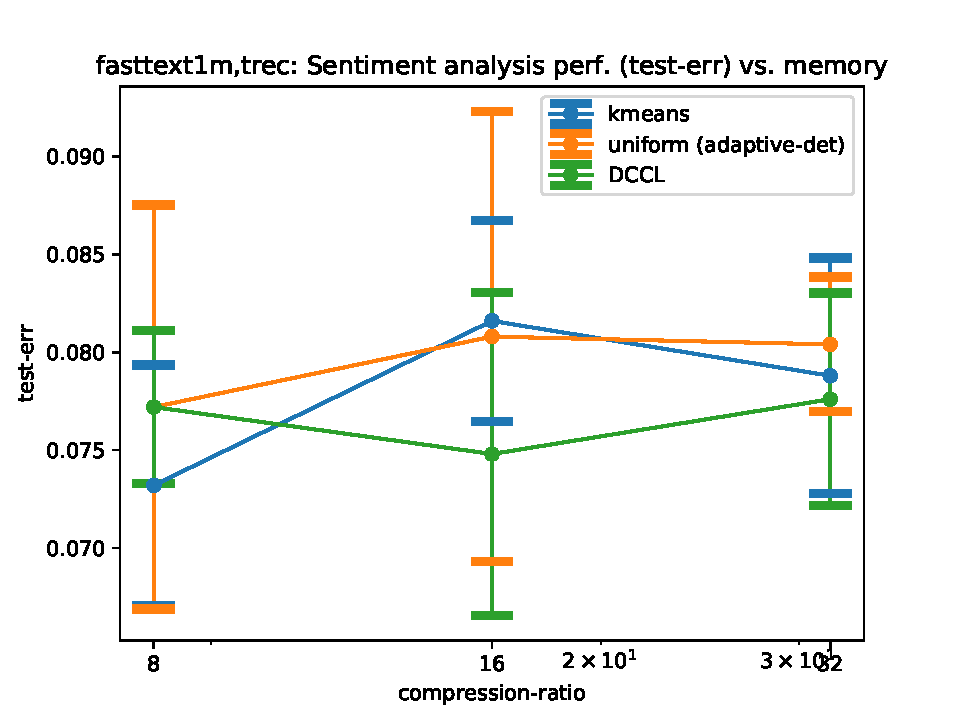
\includegraphics[width=0.28\linewidth]{figures/fasttext1m_trec_test-err_vs_compression.pdf} &
%	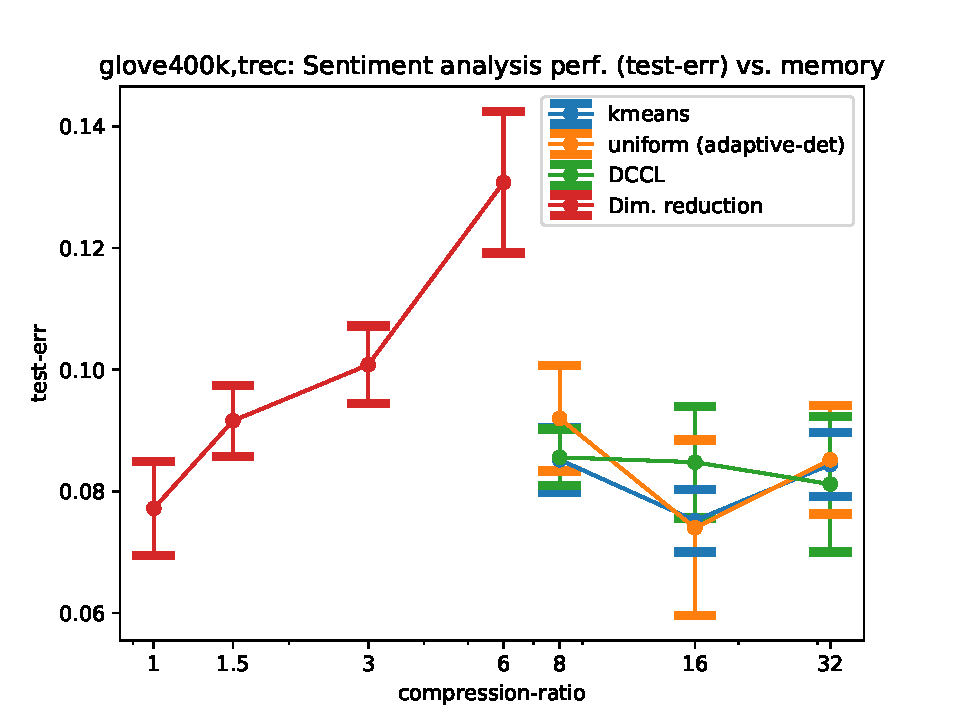
\includegraphics[width=0.28\linewidth]{figures/glove400k_trec_test-err_vs_compression.pdf} &
%	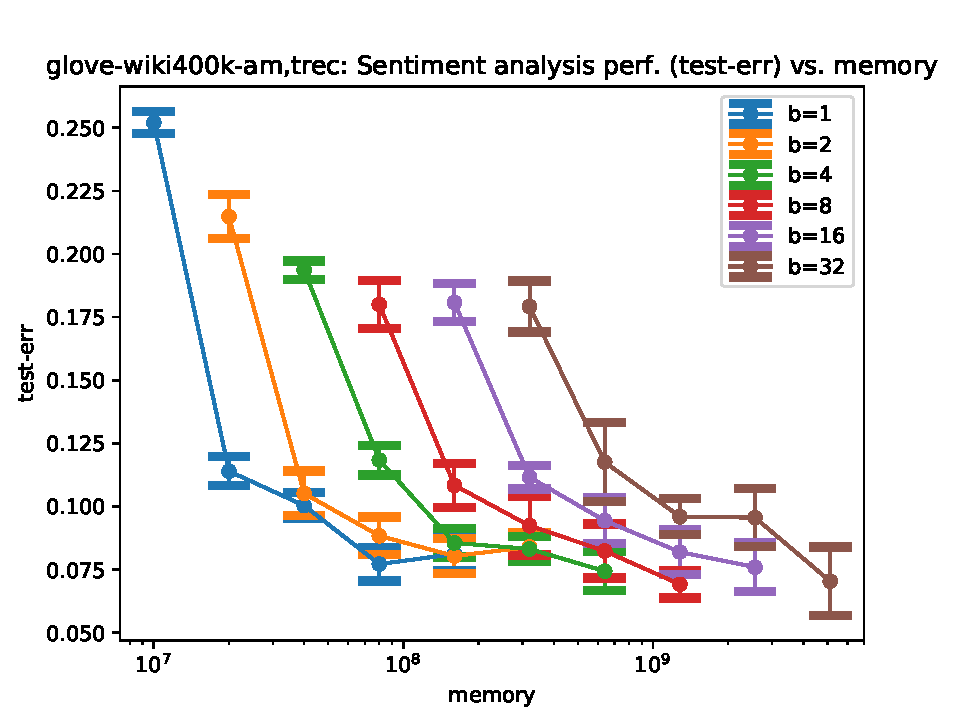
\includegraphics[width=0.28\linewidth]{figures/glove-wiki400k-am_trec_test-err_vs_compression.pdf} \\[-0.5em]
%	% SST
%	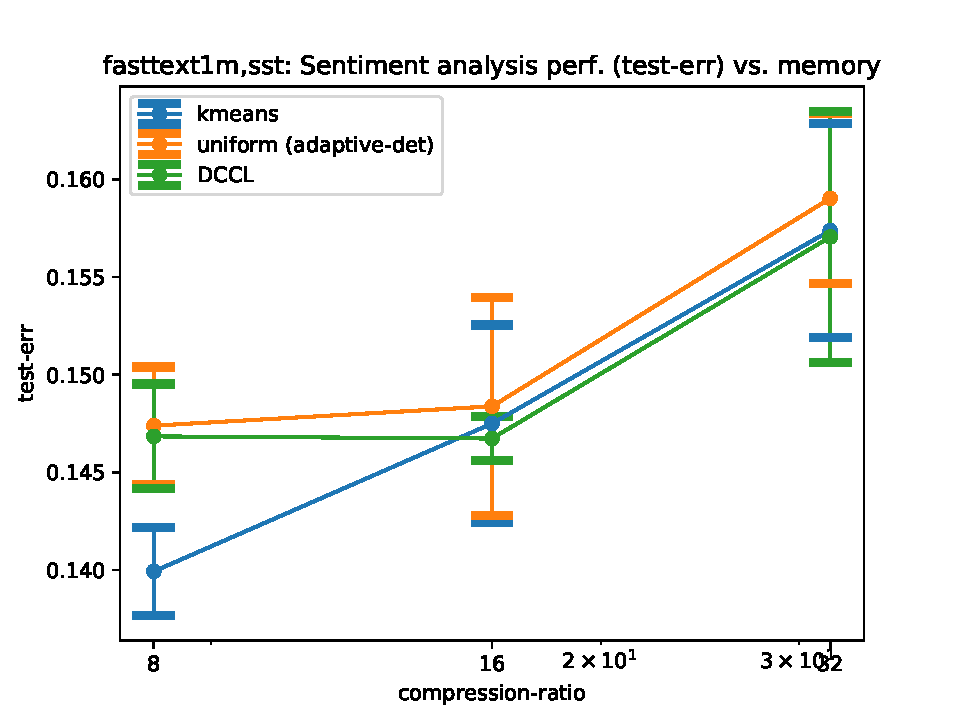
\includegraphics[width=0.28\linewidth]{figures/fasttext1m_sst_test-err_vs_compression.pdf} &
%	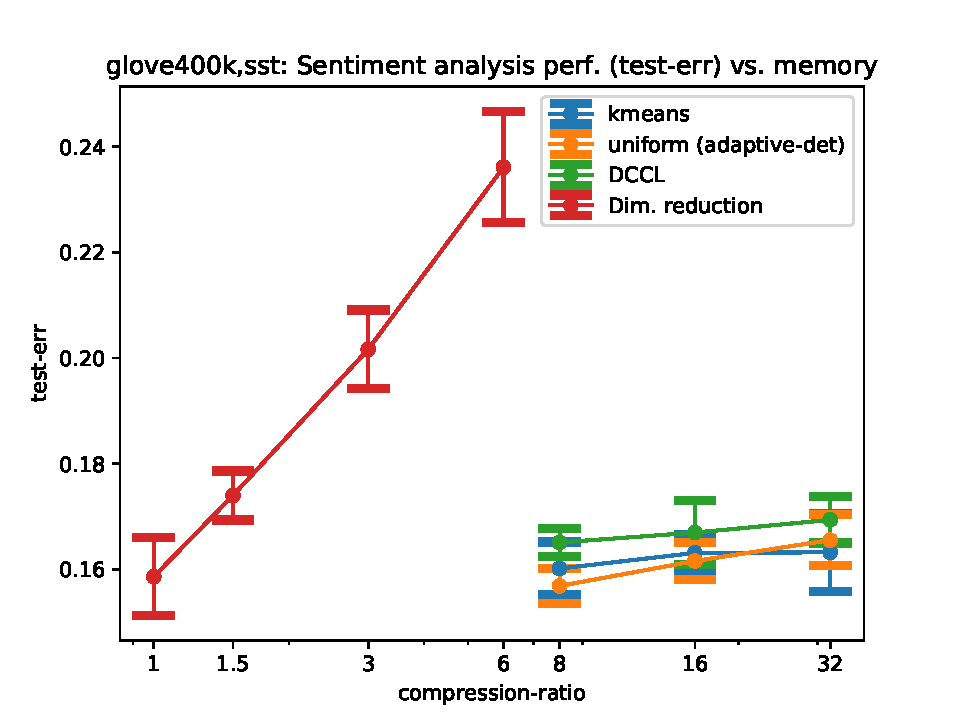
\includegraphics[width=0.28\linewidth]{figures/glove400k_sst_test-err_vs_compression.pdf} &
%	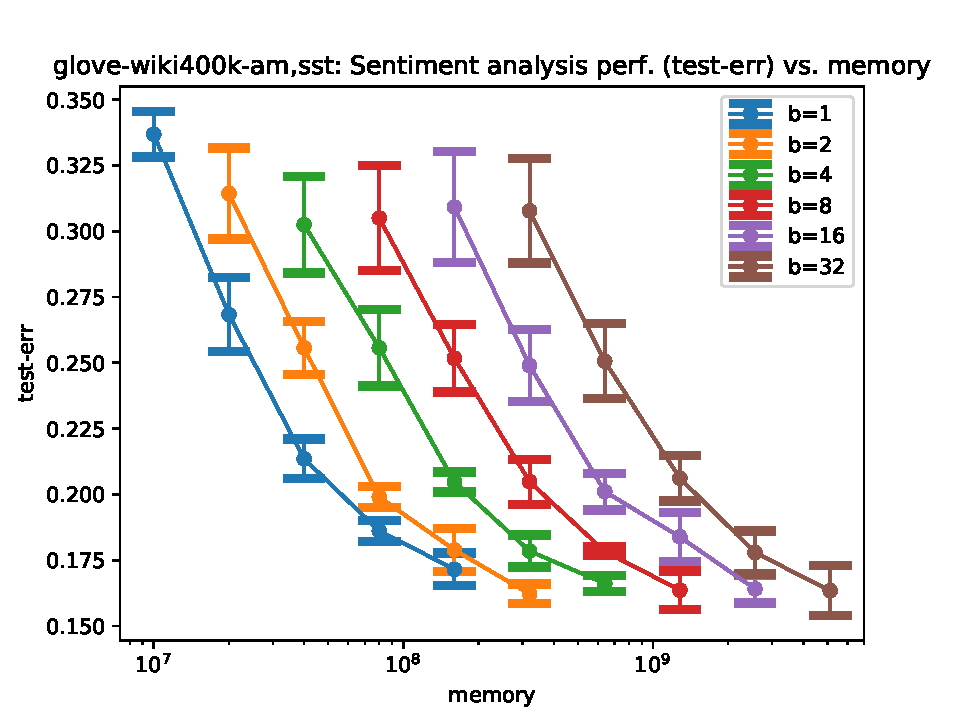
\includegraphics[width=0.28\linewidth]{figures/glove-wiki400k-am_sst_test-err_vs_compression.pdf} \\[-0.5em]
%	% CR
%	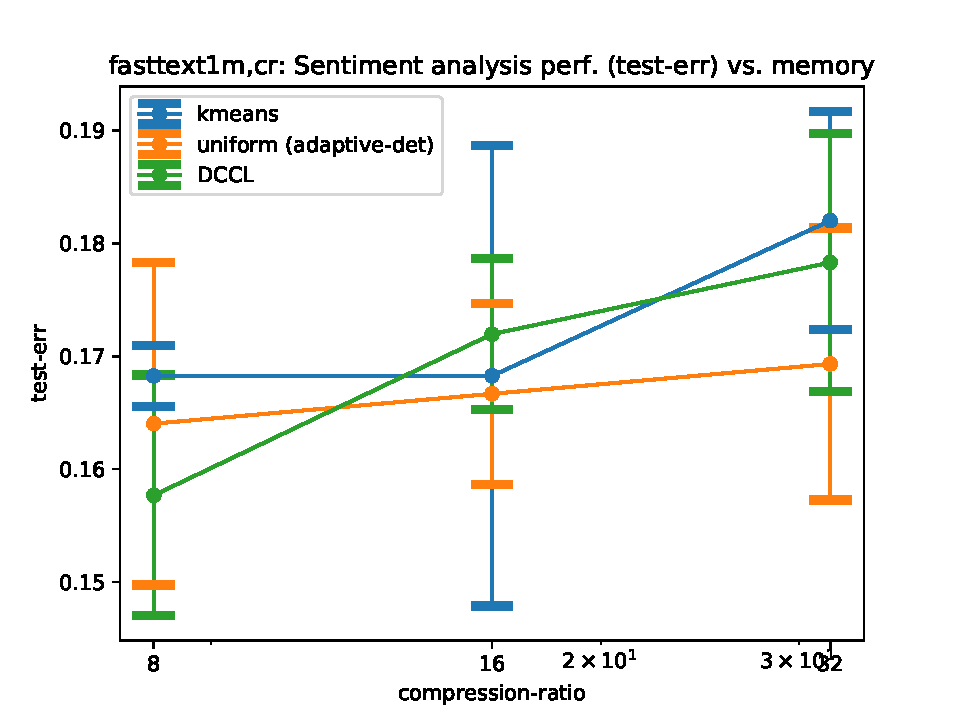
\includegraphics[width=0.28\linewidth]{figures/fasttext1m_cr_test-err_vs_compression.pdf} &
%	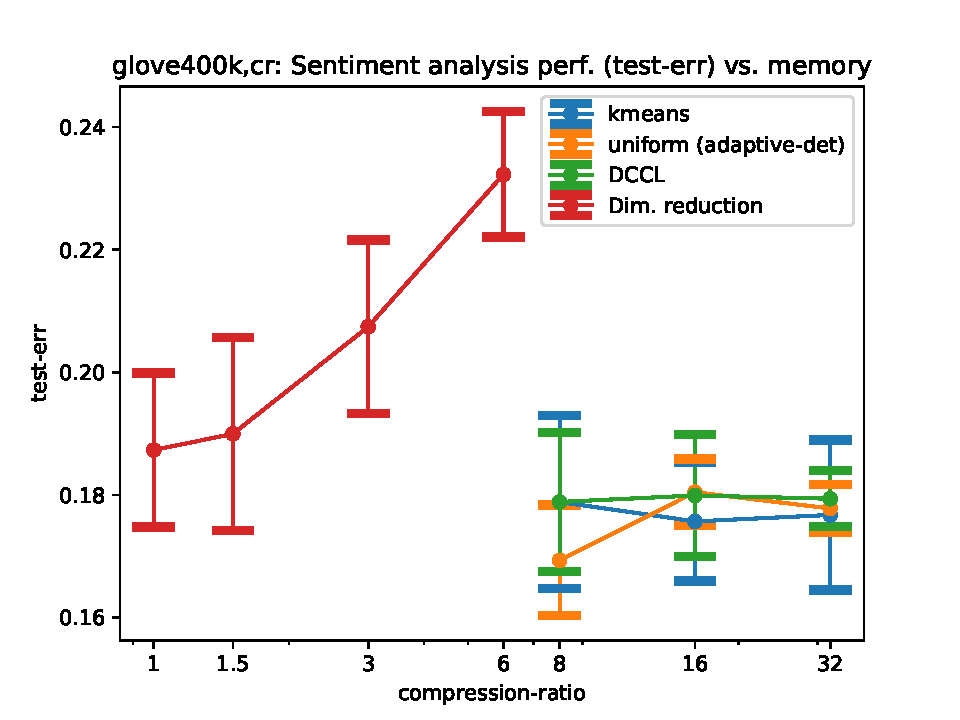
\includegraphics[width=0.28\linewidth]{figures/glove400k_cr_test-err_vs_compression.pdf} &
%	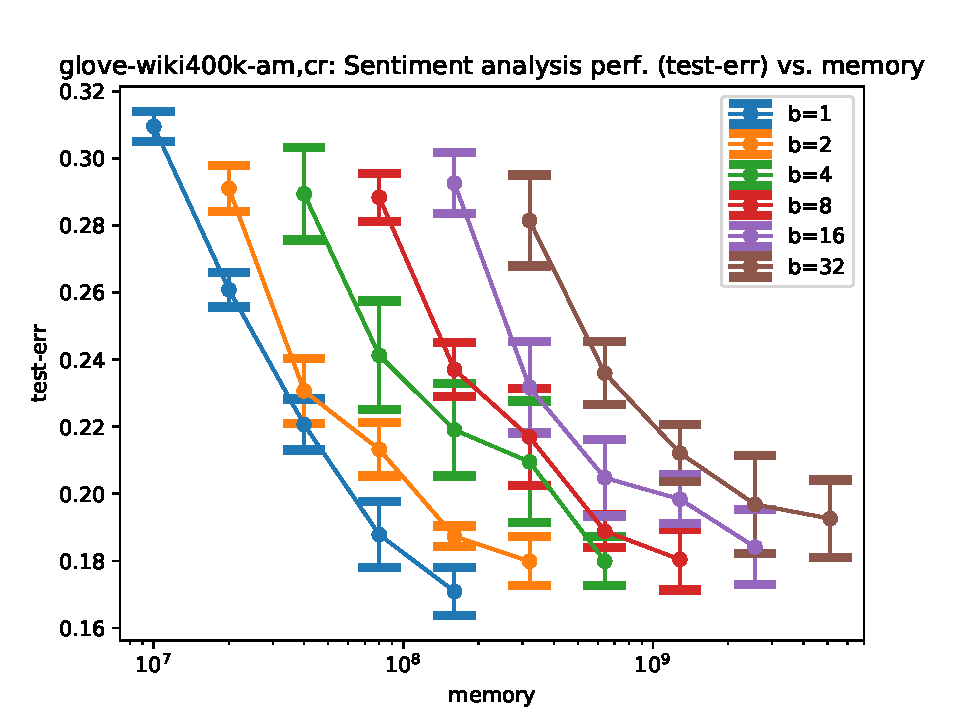
\includegraphics[width=0.28\linewidth]{figures/glove-wiki400k-am_cr_test-err_vs_compression.pdf} \\[-0.5em]
%	% SUBJ
%	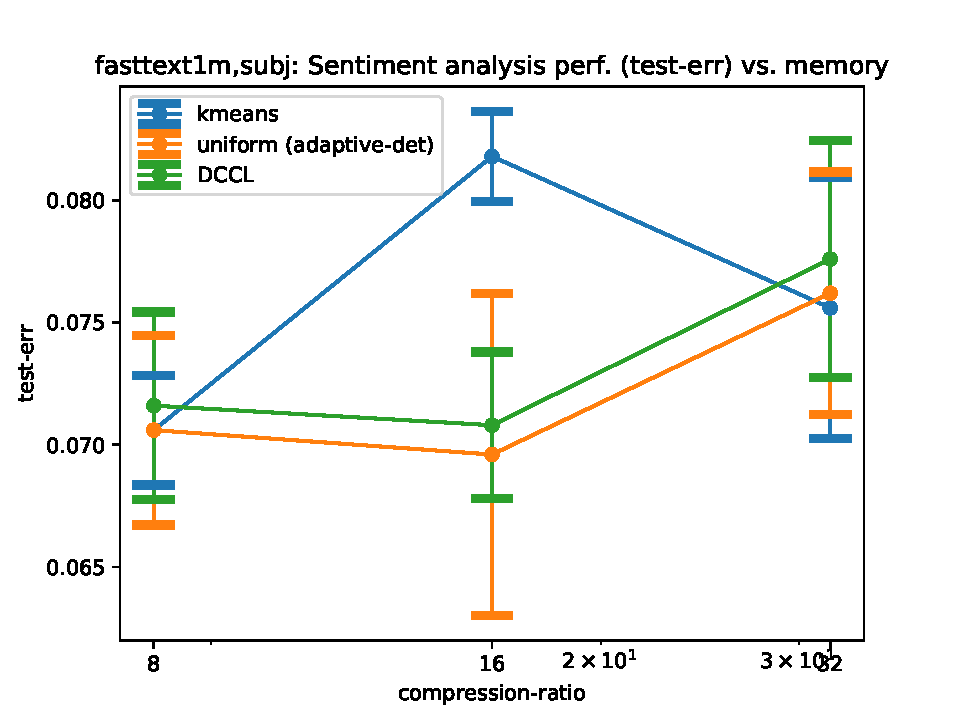
\includegraphics[width=0.28\linewidth]{figures/fasttext1m_subj_test-err_vs_compression.pdf} &
%	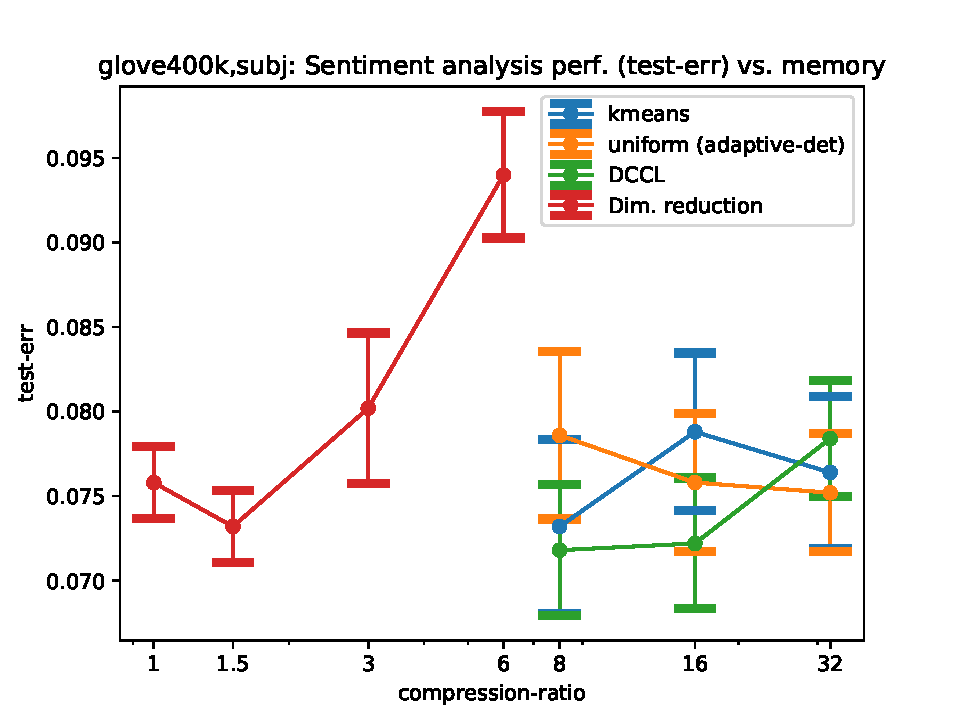
\includegraphics[width=0.28\linewidth]{figures/glove400k_subj_test-err_vs_compression.pdf} &
%	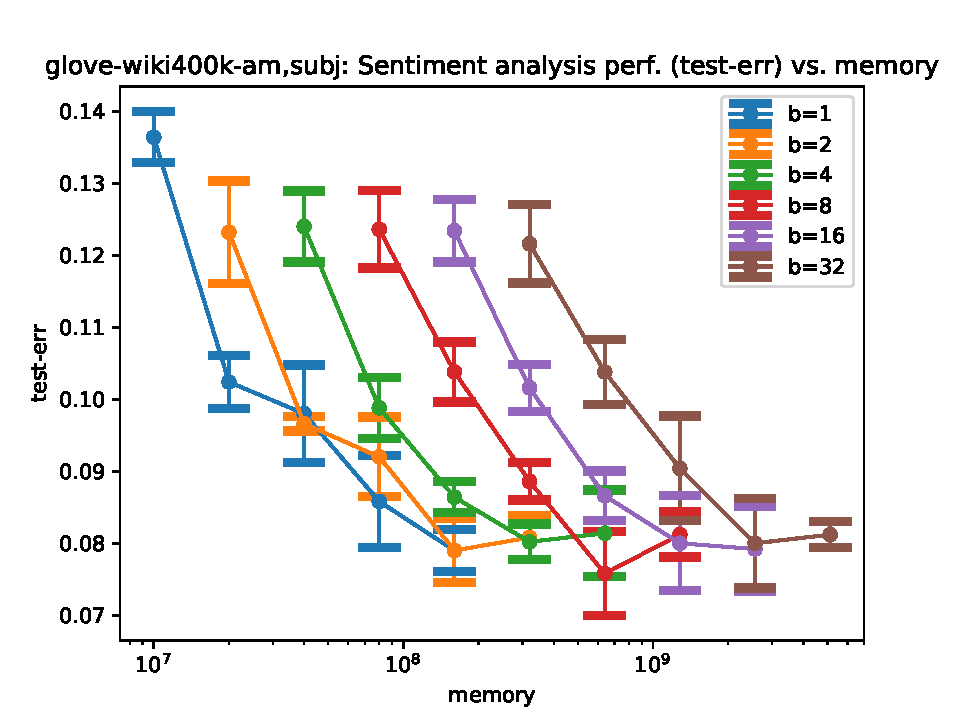
\includegraphics[width=0.28\linewidth]{figures/glove-wiki400k-am_subj_test-err_vs_compression.pdf} \\[-0.5em]
%	% MR
%	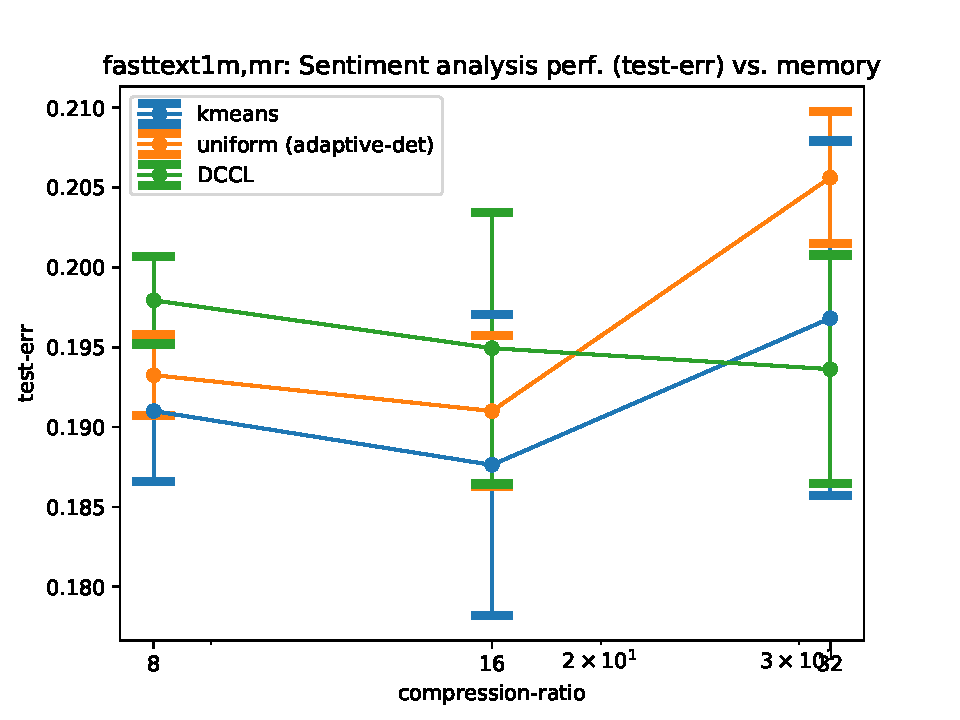
\includegraphics[width=0.28\linewidth]{figures/fasttext1m_mr_test-err_vs_compression.pdf} &
%	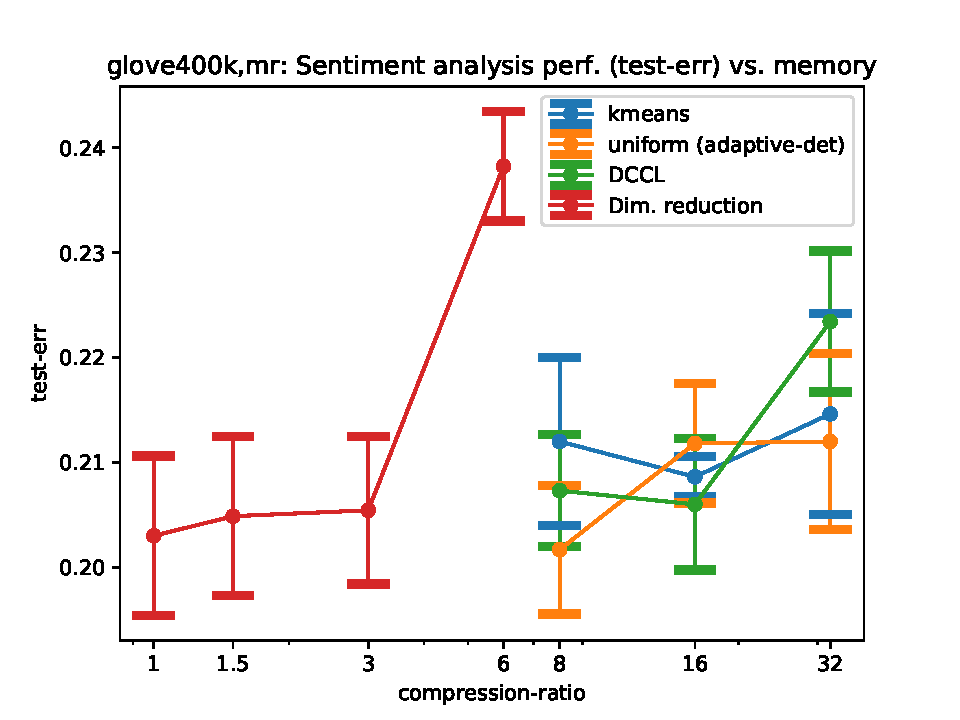
\includegraphics[width=0.28\linewidth]{figures/glove400k_mr_test-err_vs_compression.pdf} &
%	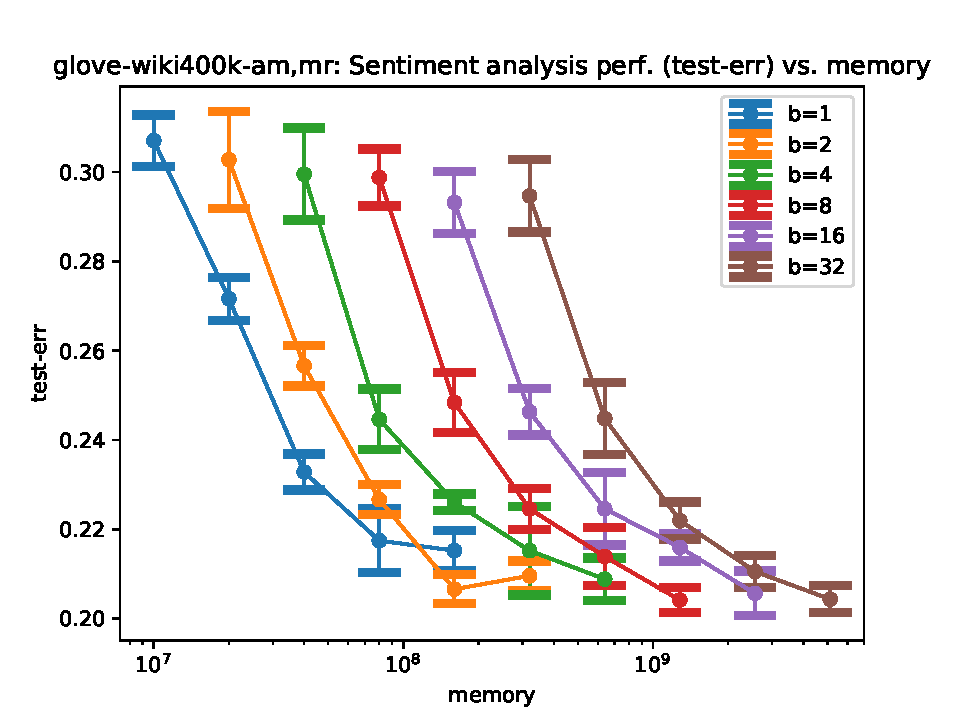
\includegraphics[width=0.28\linewidth]{figures/glove-wiki400k-am_mr_test-err_vs_compression.pdf} \\[-0.5em]
%	\end{tabular}
%	\caption{
%		Sentiment analysis results for different embeddings methods (pre-trained fastText and GloVe embeddings, and GloVe embeddings trained from scratch), on different sentiment analysis datasets (MPQA, TREC, SST, CR, SUBJ, MR).
%	}
%	\label{fig:all_sentiment}
%\end{figure}
%
%\begin{figure*}
%	\centering
%	%	\begin{tabular}{c c c c}
%	\begin{tabular}{@{\hskip -0.0in}c@{\hskip -0.0in}c@{\hskip -0.0in}c@{\hskip -0.0in}c@{\hskip -0.0in}}
%		EIG-OVERLAP & . & . & . \\
%		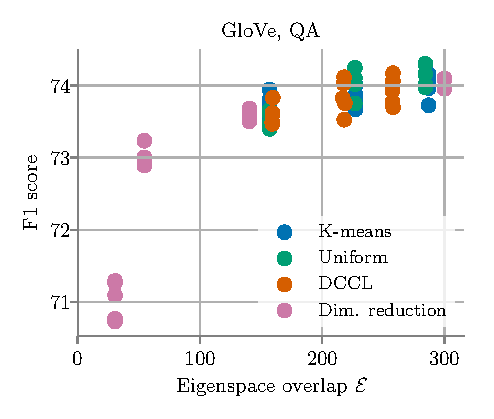
\includegraphics[width=.245\linewidth]{figures/glove400k_qa_best-f1_vs_subspace-eig-overlap_linx.pdf} &
%		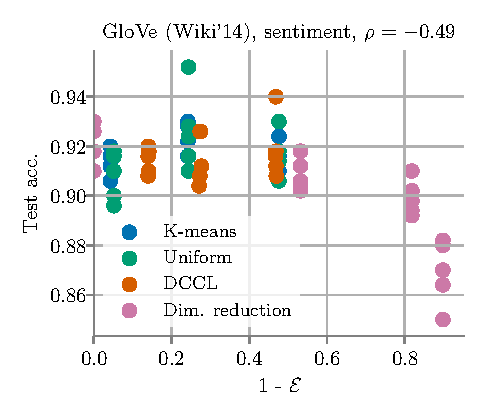
\includegraphics[width=.245\linewidth]{figures/glove400k_sentiment_trec_test-acc_vs_subspace-eig-overlap_linx.pdf} &
%		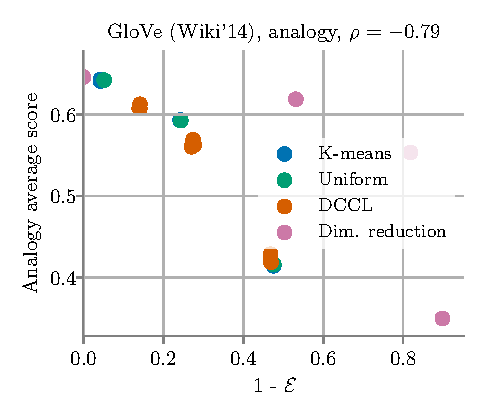
\includegraphics[width=.245\linewidth]{figures/glove400k_intrinsics_analogy-avg-score_vs_subspace-eig-overlap_linx.pdf} &
%		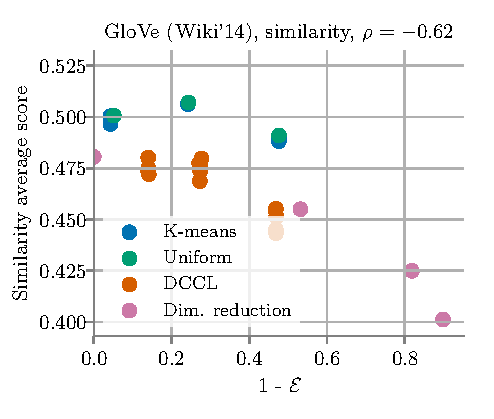
\includegraphics[width=.245\linewidth]{figures/glove400k_intrinsics_similarity-avg-score_vs_subspace-eig-overlap_linx.pdf} \\
%		
%		EIG-DISTANCE & . & . & . \\
%		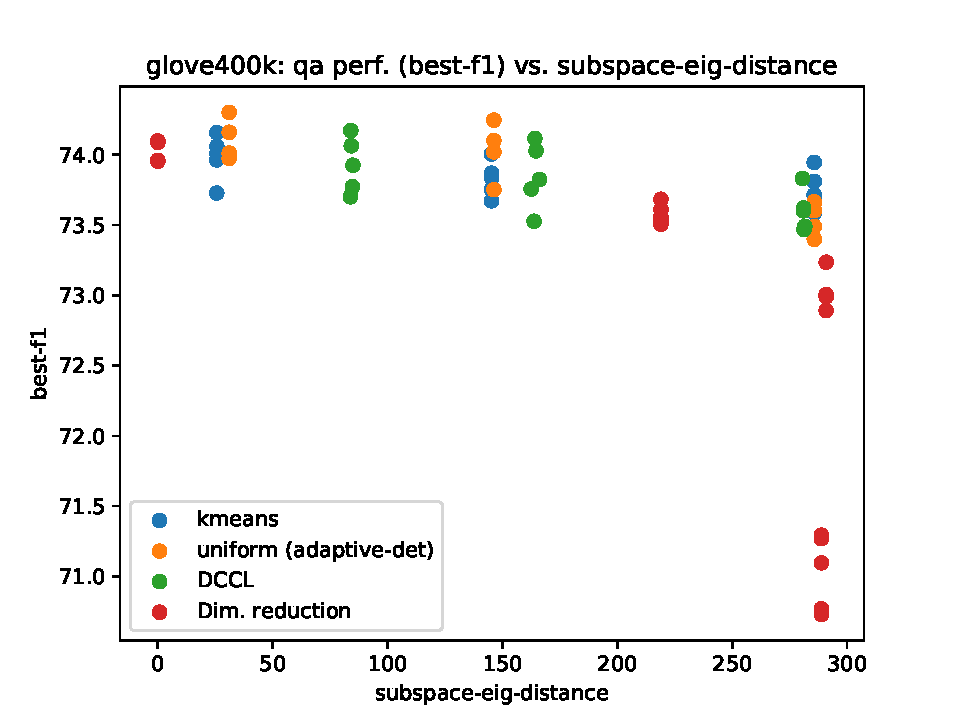
\includegraphics[width=.245\linewidth]{figures/glove400k_qa_best-f1_vs_subspace-eig-distance_linx.pdf} &
%		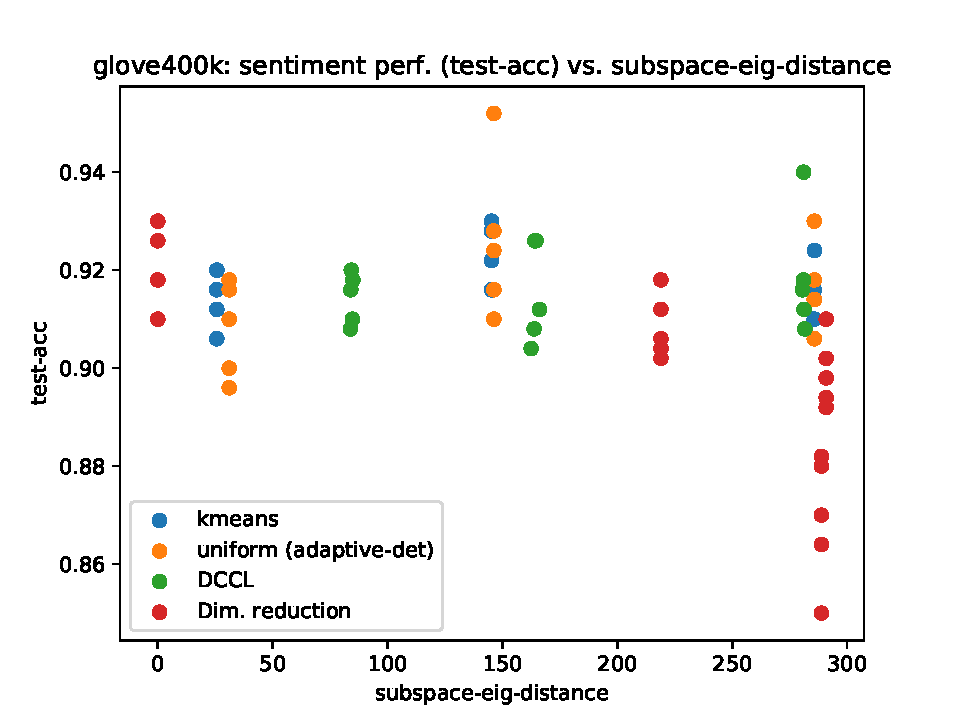
\includegraphics[width=.245\linewidth]{figures/glove400k_sentiment_trec_test-acc_vs_subspace-eig-distance_linx.pdf} &
%		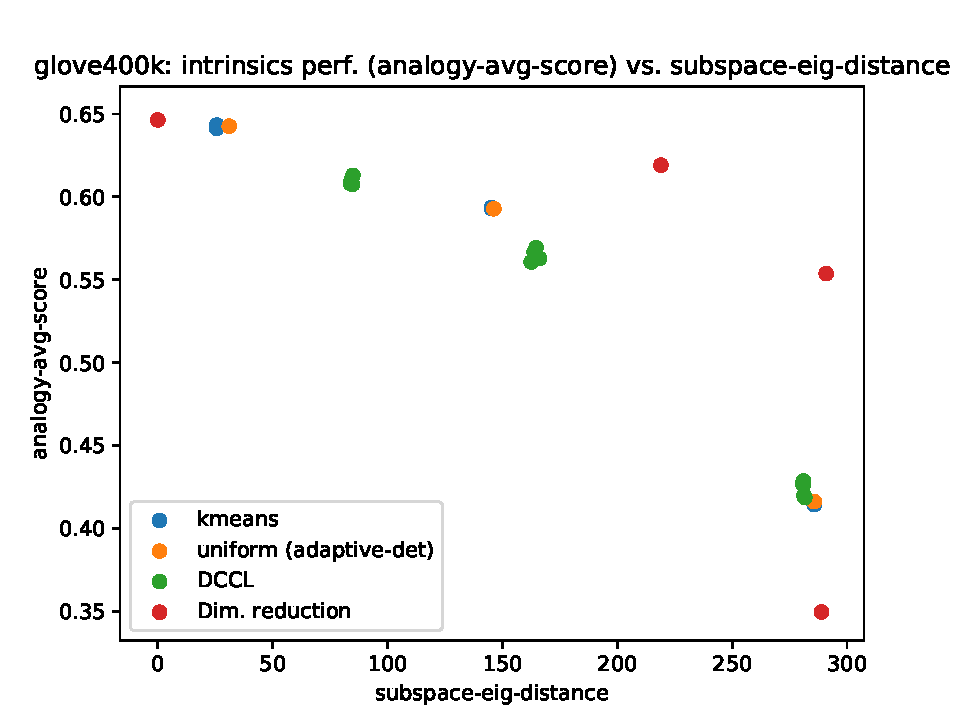
\includegraphics[width=.245\linewidth]{figures/glove400k_intrinsics_analogy-avg-score_vs_subspace-eig-distance_linx.pdf} &
%		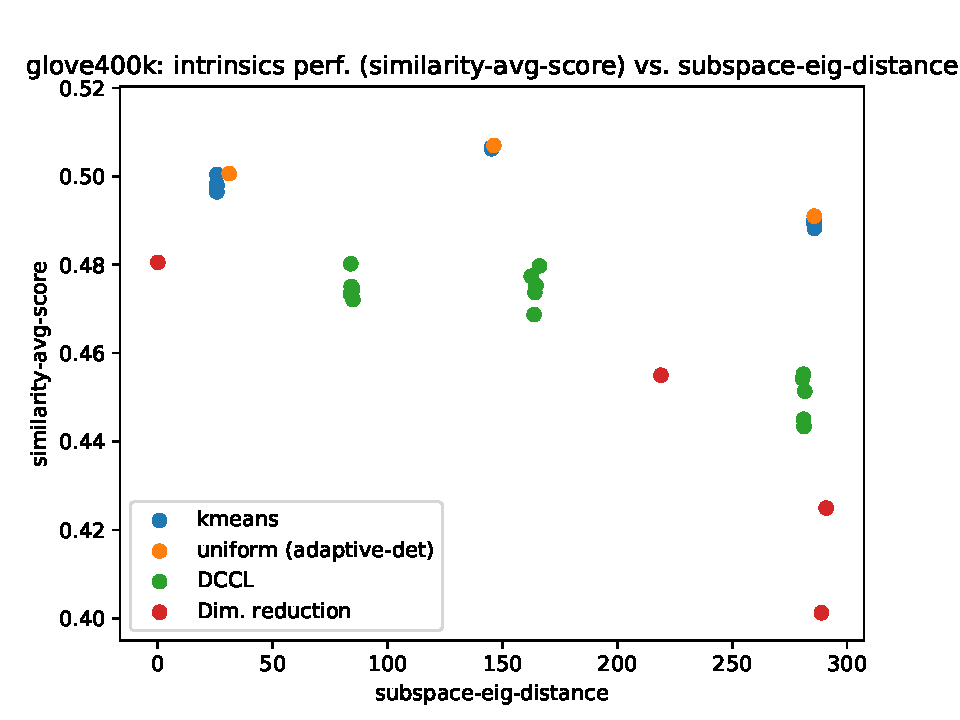
\includegraphics[width=.245\linewidth]{figures/glove400k_intrinsics_similarity-avg-score_vs_subspace-eig-distance_linx.pdf} \\
%		
%		FROBENIUS ERROR & . & . & . \\		
%		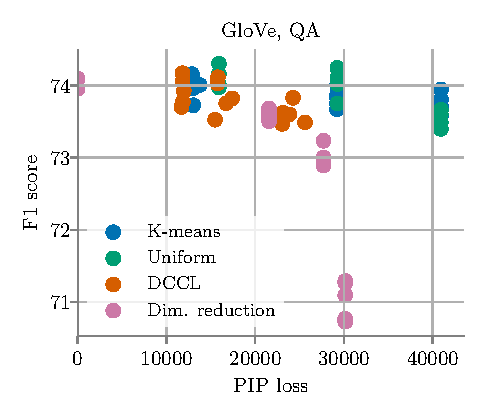
\includegraphics[width=.245\linewidth]{figures/glove400k_qa_best-f1_vs_gram-large-dim-frob-error_linx.pdf} &
%		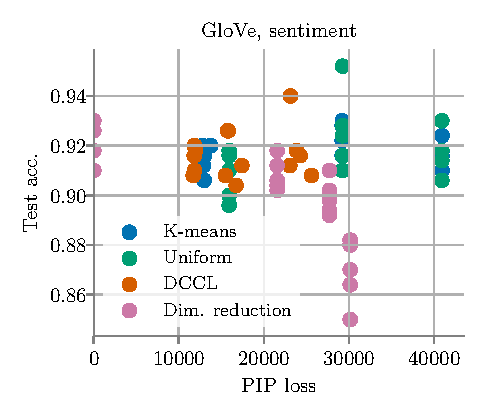
\includegraphics[width=.245\linewidth]{figures/glove400k_sentiment_trec_test-acc_vs_gram-large-dim-frob-error_linx.pdf} &
%		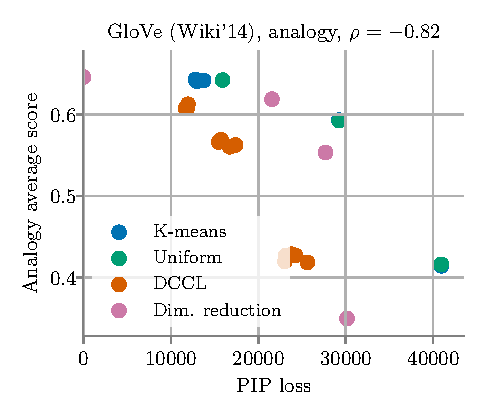
\includegraphics[width=.245\linewidth]{figures/glove400k_intrinsics_analogy-avg-score_vs_gram-large-dim-frob-error_linx.pdf} &
%		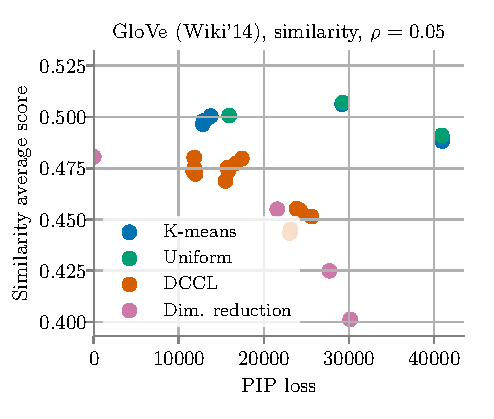
\includegraphics[width=.245\linewidth]{figures/glove400k_intrinsics_similarity-avg-score_vs_gram-large-dim-frob-error_linx.pdf} \\
%		
%		RECONSTRUCTION ERROR (FROB) & . & . & . \\		
%		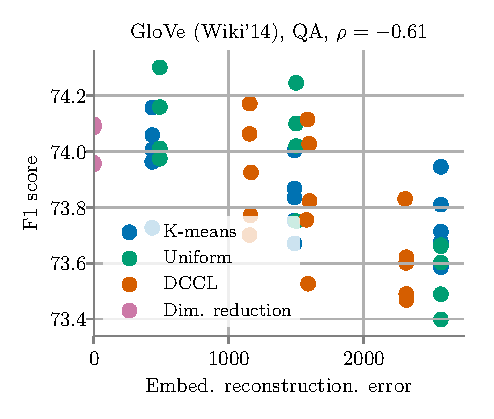
\includegraphics[width=.245\linewidth]{figures/glove400k_qa_best-f1_vs_embed-frob-error_linx.pdf} &
%		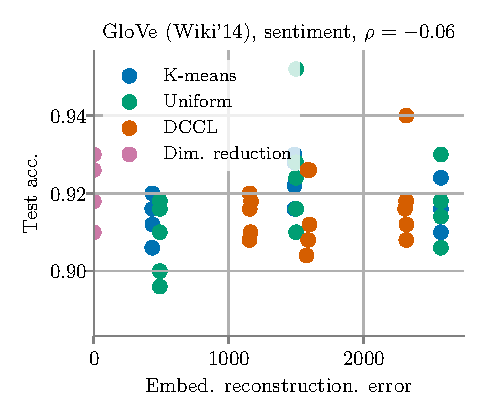
\includegraphics[width=.245\linewidth]{figures/glove400k_sentiment_trec_test-acc_vs_embed-frob-error_linx.pdf} &
%		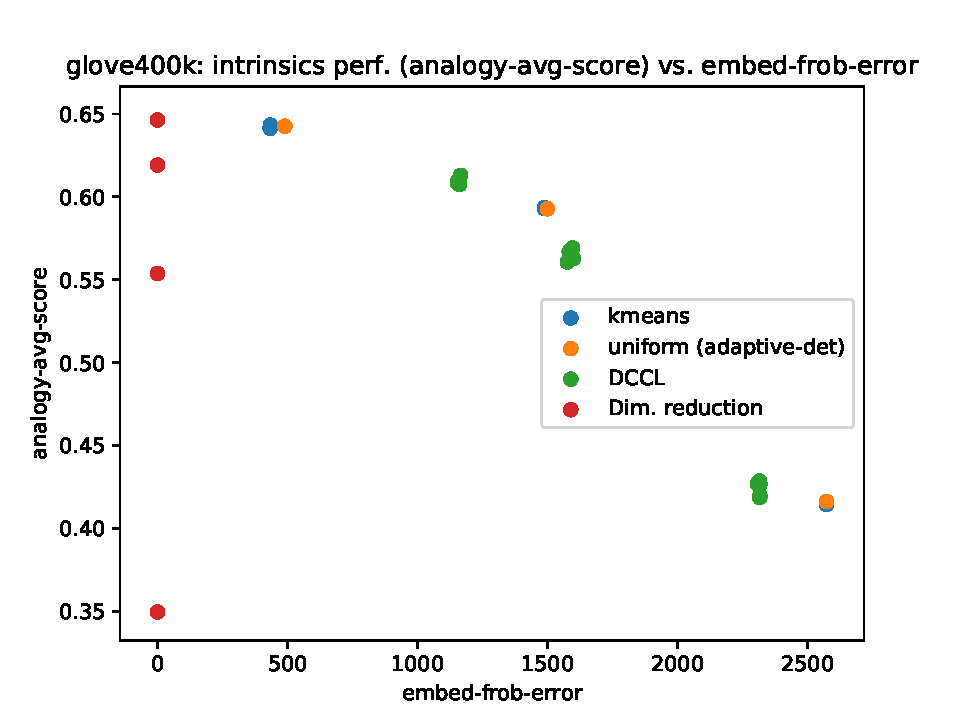
\includegraphics[width=.245\linewidth]{figures/glove400k_intrinsics_analogy-avg-score_vs_embed-frob-error_linx.pdf} &
%		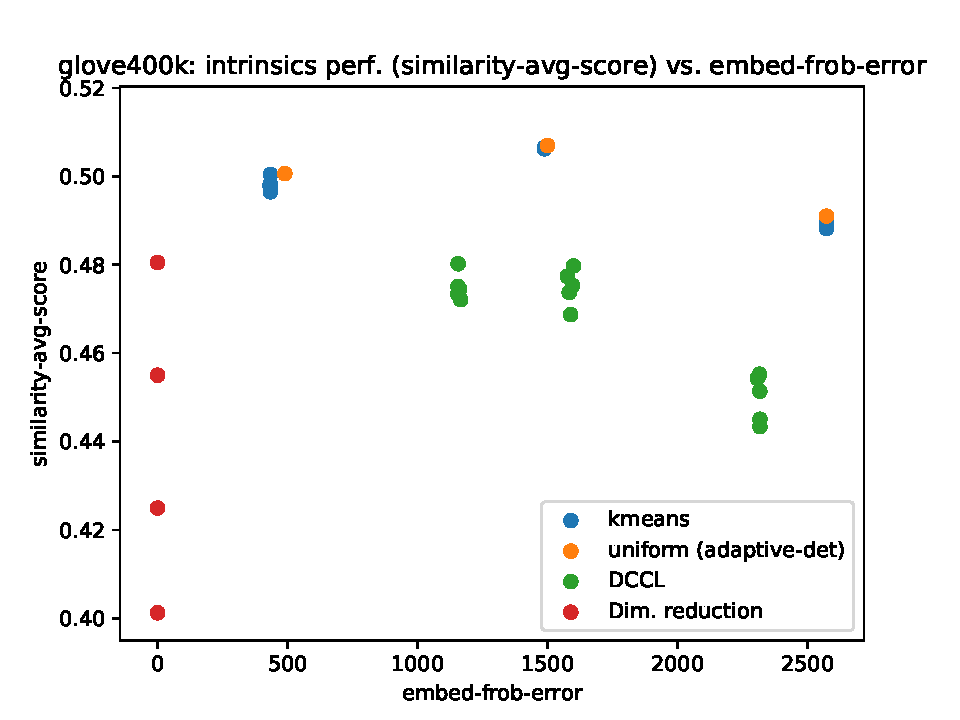
\includegraphics[width=.245\linewidth]{figures/glove400k_intrinsics_similarity-avg-score_vs_embed-frob-error_linx.pdf} \\
%		
%		
%		%DELTA1 (Lambda = sigma min/100) & . & . & . \\
%		%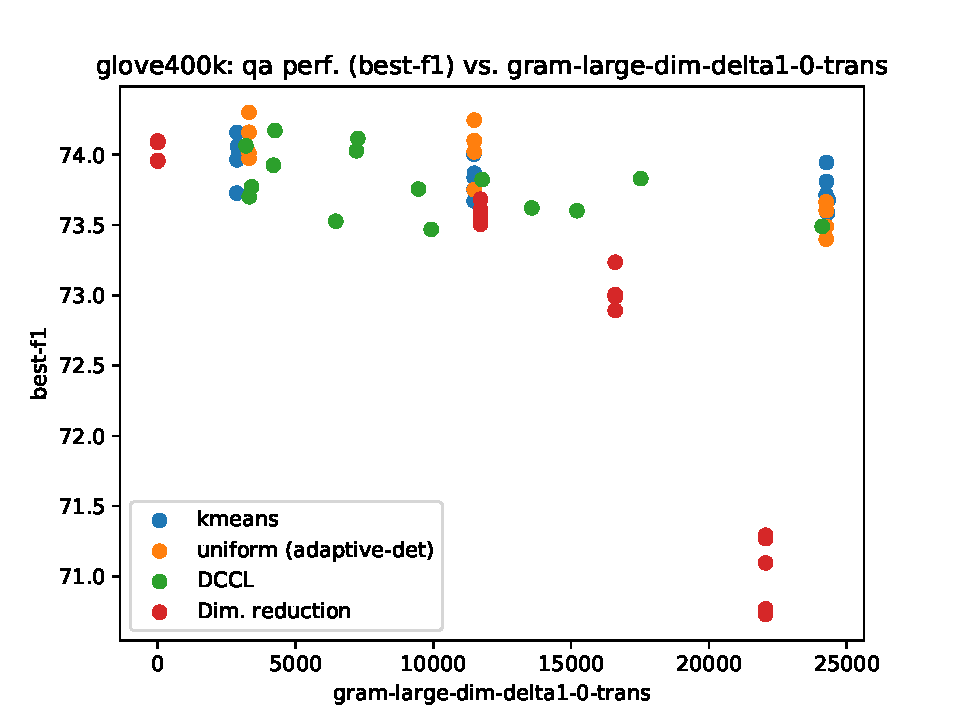
\includegraphics[width=.245\linewidth]{figures/glove400k_qa_best-f1_vs_gram-large-dim-delta1-0-trans_linx.pdf} &
%		%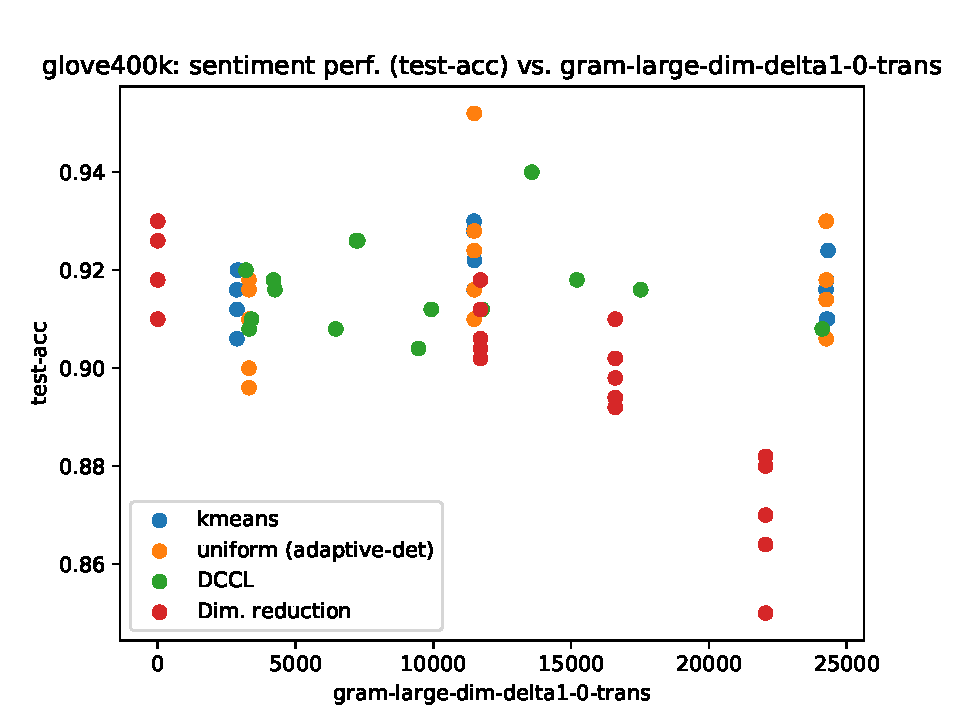
\includegraphics[width=.245\linewidth]{figures/glove400k_sentiment_trec_test-acc_vs_gram-large-dim-delta1-0-trans_linx.pdf} &
%		%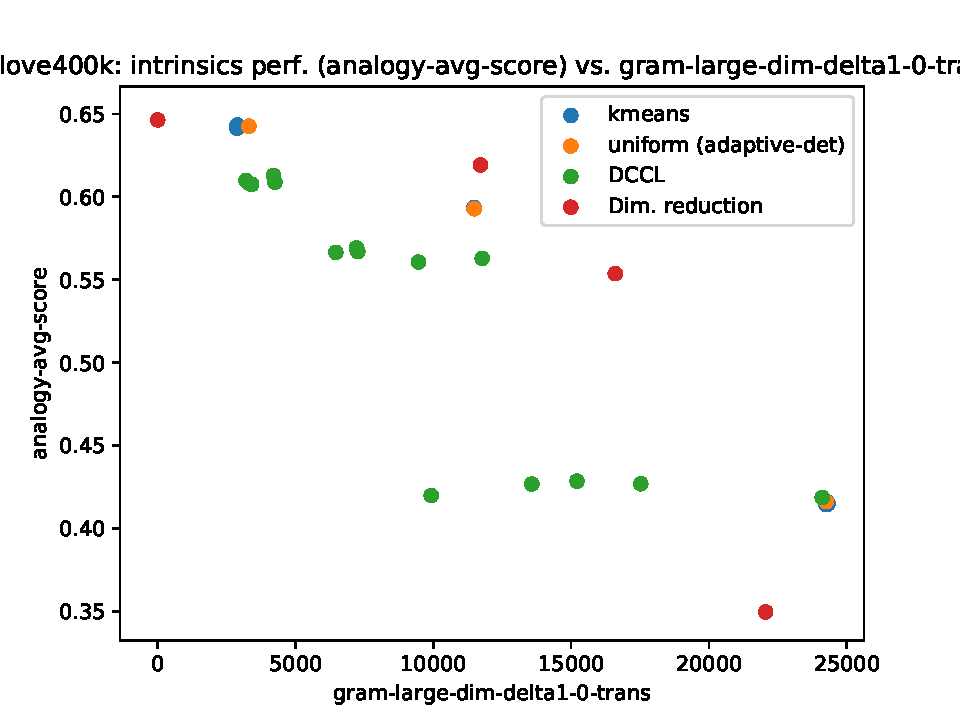
\includegraphics[width=.245\linewidth]{figures/glove400k_intrinsics_analogy-avg-score_vs_gram-large-dim-delta1-0-trans_linx.pdf} &
%		%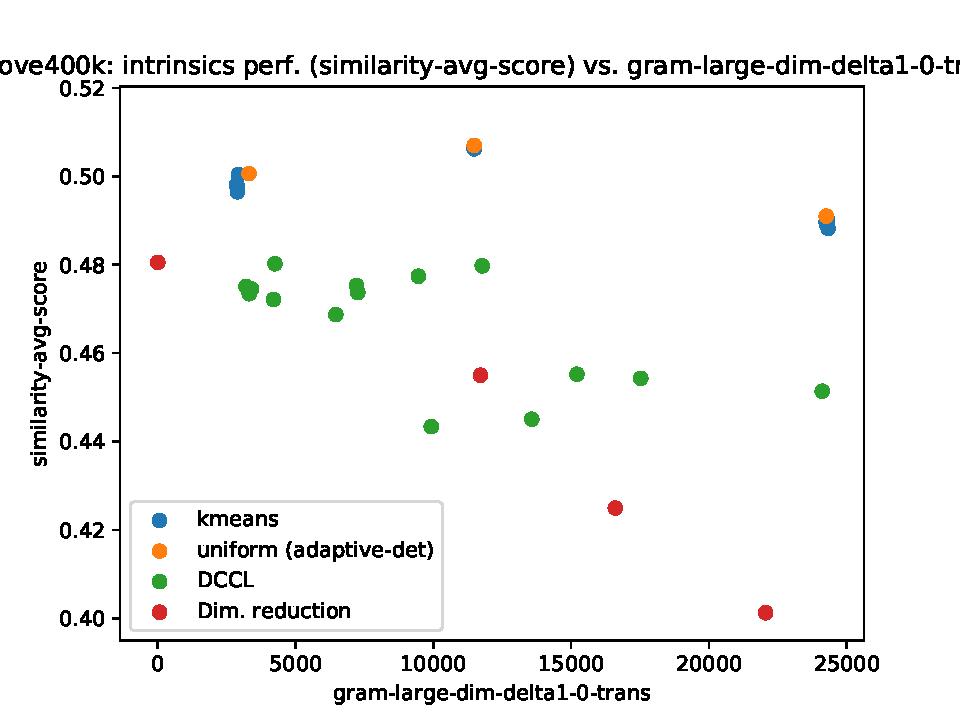
\includegraphics[width=.245\linewidth]{figures/glove400k_intrinsics_similarity-avg-score_vs_gram-large-dim-delta1-0-trans_linx.pdf} \\
%		
%		DELTA1 (Lambda = sigma min) & . & . & . \\
%		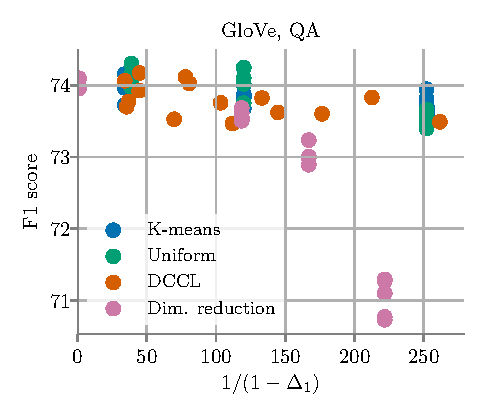
\includegraphics[width=.245\linewidth]{figures/glove400k_qa_best-f1_vs_gram-large-dim-delta1-2-trans_linx.pdf} &
%		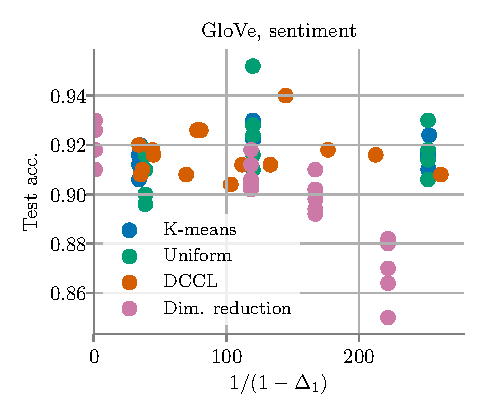
\includegraphics[width=.245\linewidth]{figures/glove400k_sentiment_trec_test-acc_vs_gram-large-dim-delta1-2-trans_linx.pdf} &
%		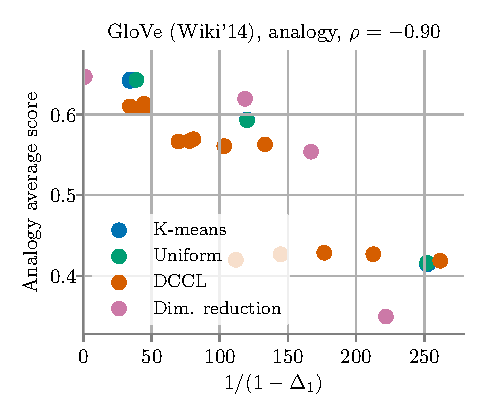
\includegraphics[width=.245\linewidth]{figures/glove400k_intrinsics_analogy-avg-score_vs_gram-large-dim-delta1-2-trans_linx.pdf} &
%		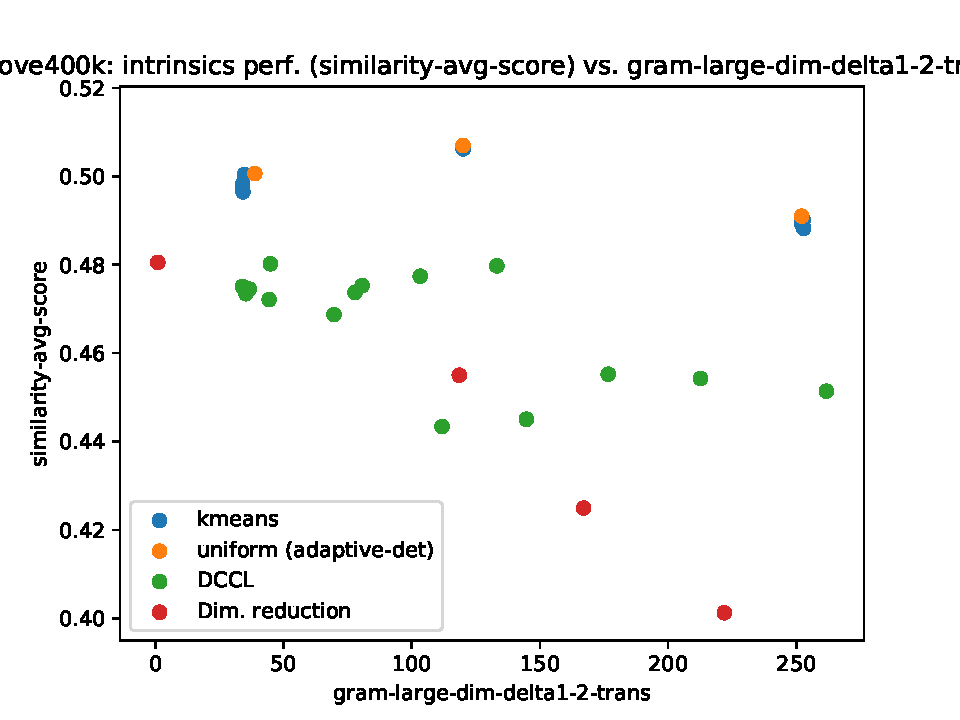
\includegraphics[width=.245\linewidth]{figures/glove400k_intrinsics_similarity-avg-score_vs_gram-large-dim-delta1-2-trans_linx.pdf} \\		
%		
%		DELTA1 (lambda = sigma max) & . & . & . \\
%		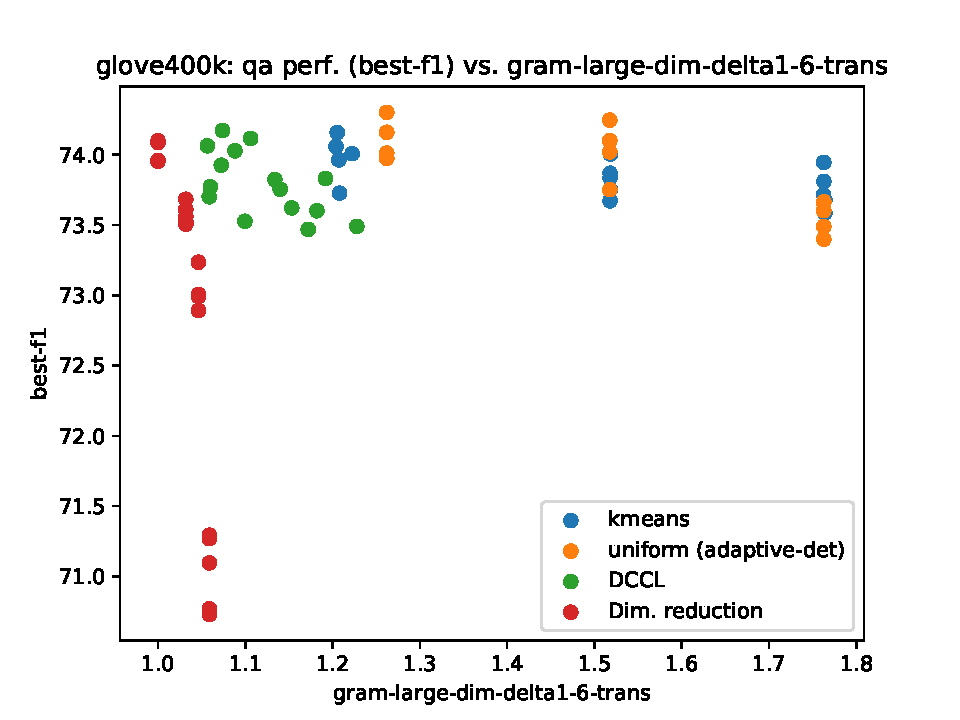
\includegraphics[width=.245\linewidth]{figures/glove400k_qa_best-f1_vs_gram-large-dim-delta1-6-trans_linx.pdf} &
%		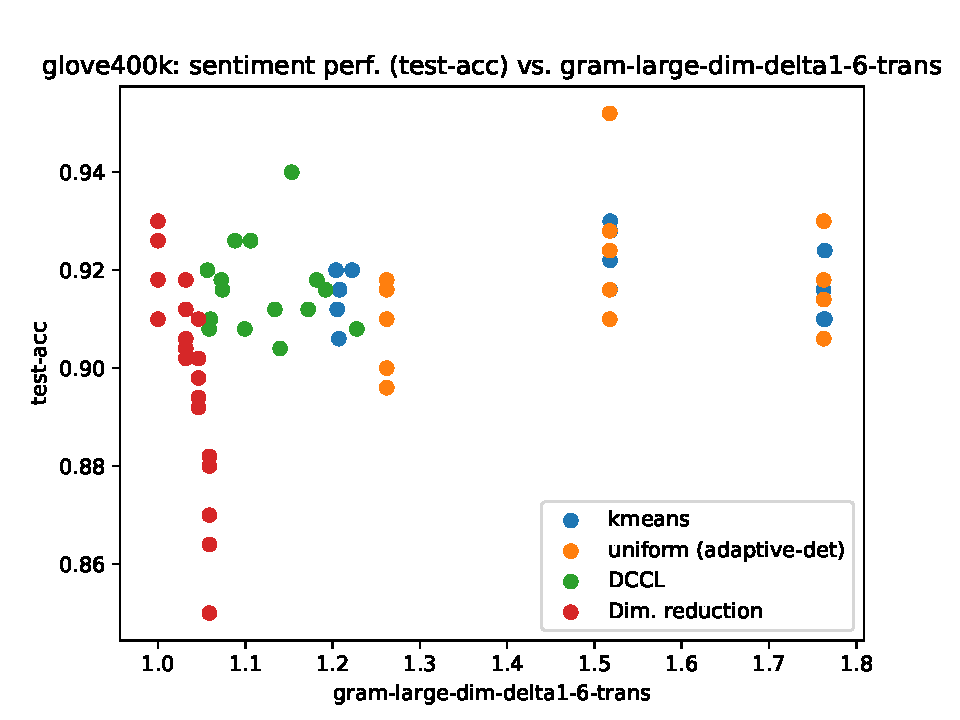
\includegraphics[width=.245\linewidth]{figures/glove400k_sentiment_trec_test-acc_vs_gram-large-dim-delta1-6-trans_linx.pdf} &
%		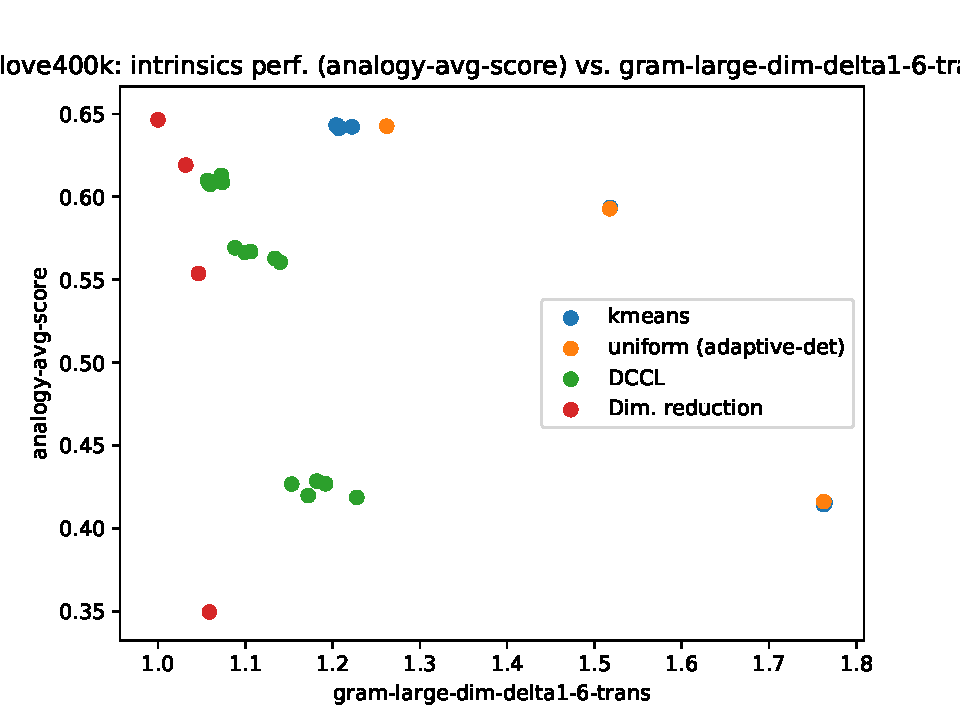
\includegraphics[width=.245\linewidth]{figures/glove400k_intrinsics_analogy-avg-score_vs_gram-large-dim-delta1-6-trans_linx.pdf} &
%		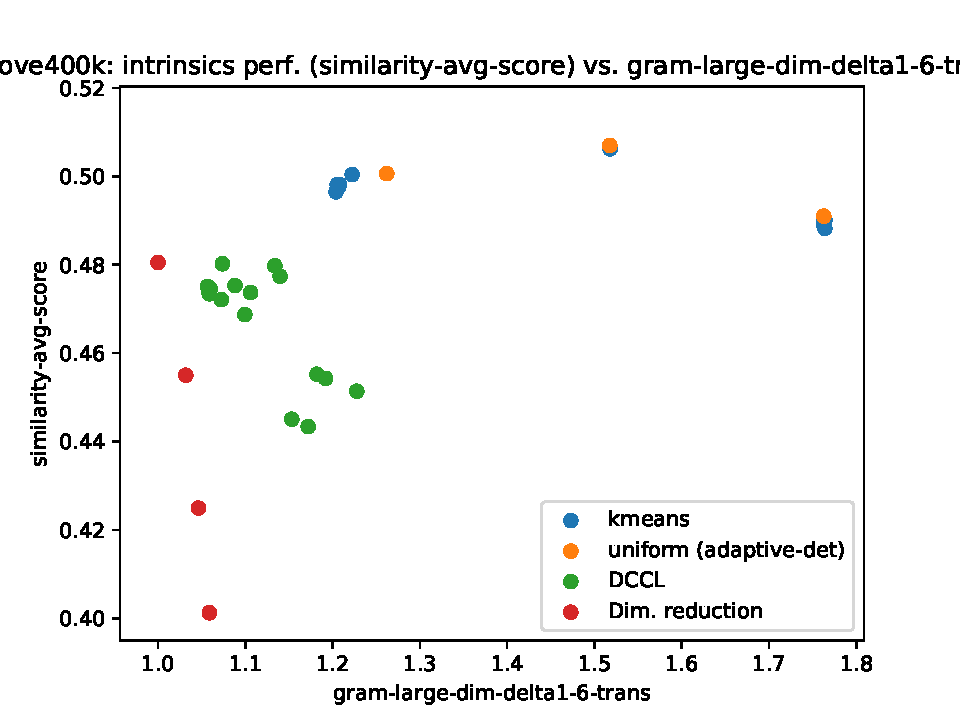
\includegraphics[width=.245\linewidth]{figures/glove400k_intrinsics_similarity-avg-score_vs_gram-large-dim-delta1-6-trans_linx.pdf} \\		
%		
%		\;\;\;\;\;(a) & \;\;\;\;\;\;(b) & \;\;\;\;\;\;(c) & \;\;\;\;\;\;(d)
%	\end{tabular}
%	\caption{GLOVE400k: Performance vs. metrics. (a) QA, (b) Sentiment (TREC), (c) Analogy average, (d) Similarity average.
%	}
%	\label{fig:glove400k_comparison_results}
%\end{figure*}
%
%
%\begin{figure*}
%	\centering
%	%	\begin{tabular}{c c c c}
%	\begin{tabular}{@{\hskip -0.0in}c@{\hskip -0.0in}c@{\hskip -0.0in}c@{\hskip -0.0in}c@{\hskip -0.0in}}
%		EIG-OVERLAP & . & . & . \\
%		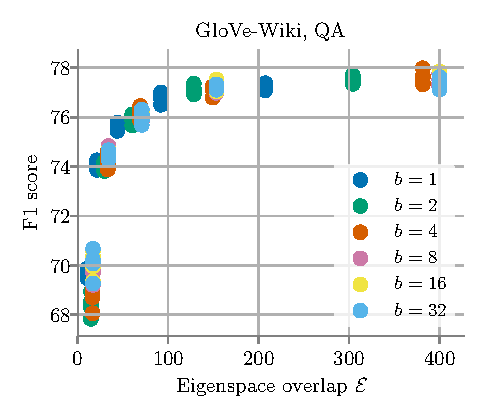
\includegraphics[width=.245\linewidth]{figures/glove-wiki400k-am_qa_best-f1_vs_subspace-eig-overlap_linx.pdf} &
%		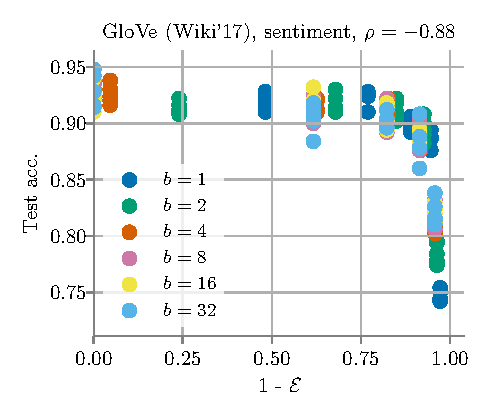
\includegraphics[width=.245\linewidth]{figures/glove-wiki400k-am_sentiment_trec_test-acc_vs_subspace-eig-overlap_linx.pdf} &
%		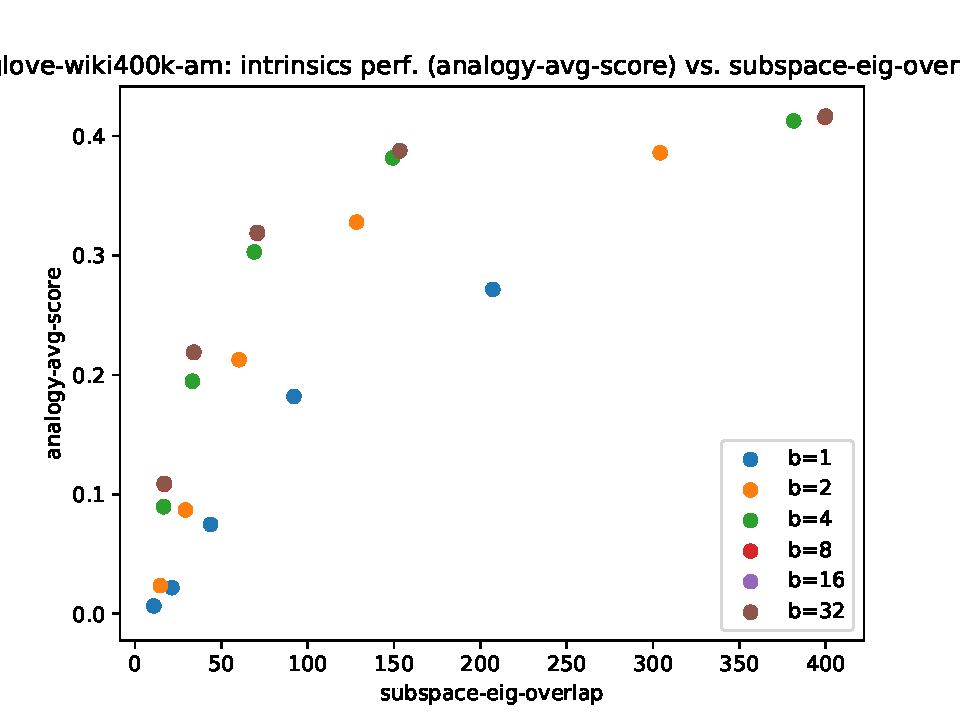
\includegraphics[width=.245\linewidth]{figures/glove-wiki400k-am_intrinsics_analogy-avg-score_vs_subspace-eig-overlap_linx.pdf} &
%		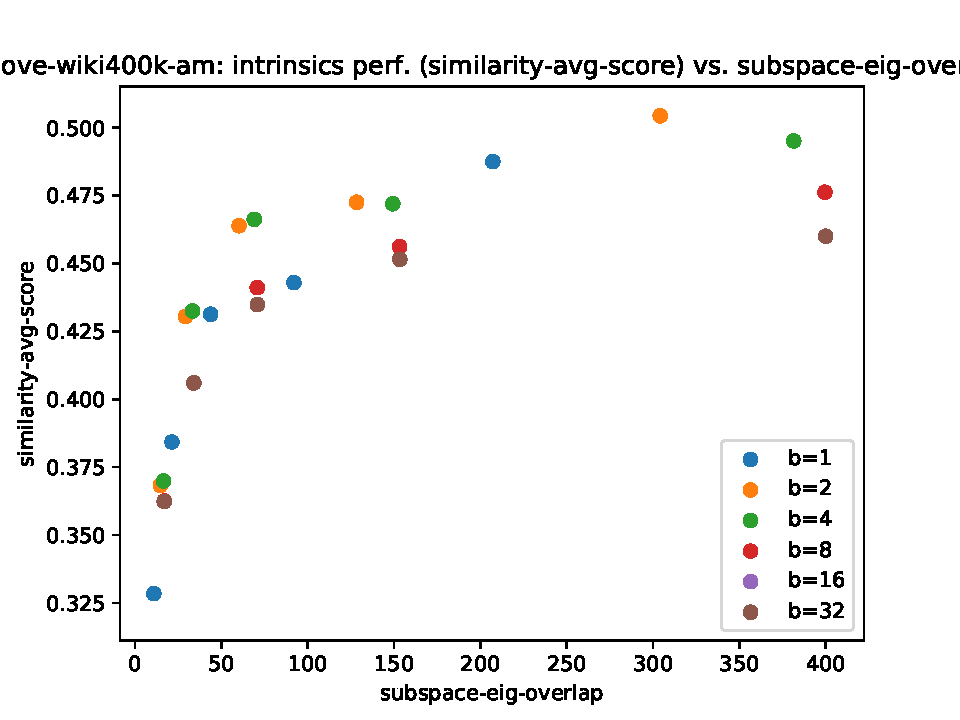
\includegraphics[width=.245\linewidth]{figures/glove-wiki400k-am_intrinsics_similarity-avg-score_vs_subspace-eig-overlap_linx.pdf} \\
%		
%		EIG-DISTANCE & . & . & . \\
%		\includegraphics[width=.245\linewidth]{figures/glove-wiki400k-am_qa_best-f1_vs_subspace-eig-distance_linx.pdf} &
%		\includegraphics[width=.245\linewidth]{figures/glove-wiki400k-am_sentiment_trec_test-acc_vs_subspace-eig-distance_linx.pdf} &
%		\includegraphics[width=.245\linewidth]{figures/glove-wiki400k-am_intrinsics_analogy-avg-score_vs_subspace-eig-distance_linx.pdf} &
%		\includegraphics[width=.245\linewidth]{figures/glove-wiki400k-am_intrinsics_similarity-avg-score_vs_subspace-eig-distance_linx.pdf} \\
%		
%		FROBENIUS ERROR & . & . & . \\		
%		\includegraphics[width=.245\linewidth]{figures/glove-wiki400k-am_qa_best-f1_vs_gram-large-dim-frob-error_linx.pdf} &
%		\includegraphics[width=.245\linewidth]{figures/glove-wiki400k-am_sentiment_trec_test-acc_vs_gram-large-dim-frob-error_linx.pdf} &
%		\includegraphics[width=.245\linewidth]{figures/glove-wiki400k-am_intrinsics_analogy-avg-score_vs_gram-large-dim-frob-error_linx.pdf} &
%		\includegraphics[width=.245\linewidth]{figures/glove-wiki400k-am_intrinsics_similarity-avg-score_vs_gram-large-dim-frob-error_linx.pdf} \\
%		
%		
%		RECONSTRUCTION ERROR (FROB) & . & . & . \\		
%		\includegraphics[width=.245\linewidth]{figures/glove-wiki400k-am_qa_best-f1_vs_embed-frob-error_linx.pdf} &
%		\includegraphics[width=.245\linewidth]{figures/glove-wiki400k-am_sentiment_trec_test-acc_vs_embed-frob-error_linx.pdf} &
%		\includegraphics[width=.245\linewidth]{figures/glove-wiki400k-am_intrinsics_analogy-avg-score_vs_embed-frob-error_linx.pdf} &
%		\includegraphics[width=.245\linewidth]{figures/glove-wiki400k-am_intrinsics_similarity-avg-score_vs_embed-frob-error_linx.pdf} \\
%		%		DELTA1 (Lambda = sigma min/100) & . & . & . \\
%		%		\includegraphics[width=.245\linewidth]{figures/glove-wiki400k-am_qa_best-f1_vs_gram-large-dim-delta1-0-trans_linx.pdf} &
%		%		\includegraphics[width=.245\linewidth]{figures/glove-wiki400k-am_sentiment_trec_test-acc_vs_gram-large-dim-delta1-0-trans_linx.pdf} &
%		%		\includegraphics[width=.245\linewidth]{figures/glove-wiki400k-am_intrinsics_analogy-avg-score_vs_gram-large-dim-delta1-0-trans_linx.pdf} &
%		%		\includegraphics[width=.245\linewidth]{figures/glove-wiki400k-am_intrinsics_similarity-avg-score_vs_gram-large-dim-delta1-0-trans_linx.pdf} \\		
%		
%		DELTA1 (Lambda = sigma min) & . & . & . \\
%		\includegraphics[width=.245\linewidth]{figures/glove-wiki400k-am_qa_best-f1_vs_gram-large-dim-delta1-2-trans_linx.pdf} &
%		\includegraphics[width=.245\linewidth]{figures/glove-wiki400k-am_sentiment_trec_test-acc_vs_gram-large-dim-delta1-2-trans_linx.pdf} &
%		\includegraphics[width=.245\linewidth]{figures/glove-wiki400k-am_intrinsics_analogy-avg-score_vs_gram-large-dim-delta1-2-trans_linx.pdf} &
%		\includegraphics[width=.245\linewidth]{figures/glove-wiki400k-am_intrinsics_similarity-avg-score_vs_gram-large-dim-delta1-2-trans_linx.pdf} \\		
%		
%		DELTA1 (lambda = sigma max) & . & . & . \\
%		\includegraphics[width=.245\linewidth]{figures/glove-wiki400k-am_qa_best-f1_vs_gram-large-dim-delta1-6-trans_linx.pdf} &
%		\includegraphics[width=.245\linewidth]{figures/glove-wiki400k-am_sentiment_trec_test-acc_vs_gram-large-dim-delta1-6-trans_linx.pdf} &
%		\includegraphics[width=.245\linewidth]{figures/glove-wiki400k-am_intrinsics_analogy-avg-score_vs_gram-large-dim-delta1-6-trans_linx.pdf} &
%		\includegraphics[width=.245\linewidth]{figures/glove-wiki400k-am_intrinsics_similarity-avg-score_vs_gram-large-dim-delta1-6-trans_linx.pdf} \\		
%		
%		\;\;\;\;\;(a) & \;\;\;\;\;\;(b) & \;\;\;\;\;\;(c) & \;\;\;\;\;\;(d)
%	\end{tabular}
%	\caption{glove-wiki400k-am: Performance vs. metrics. (a) QA, (b) Sentiment (TREC), (c) Analogy average, (d) Similarity average.
%	}
%	\label{fig:glove_wiki400k_am_comparison_results}
%\end{figure*}
%
%
%\begin{figure*}
%	\centering
%	%	\begin{tabular}{c c c c}
%	\begin{tabular}{@{\hskip -0.0in}c@{\hskip -0.0in}c@{\hskip -0.0in}c@{\hskip -0.0in}c@{\hskip -0.0in}}
%		EIG-OVERLAP & . & . & . \\
%		\includegraphics[width=.245\linewidth]{figures/fasttext1m_qa_best-f1_vs_subspace-eig-overlap_linx.pdf} &
%		\includegraphics[width=.245\linewidth]{figures/fasttext1m_sentiment_trec_test-acc_vs_subspace-eig-overlap_linx.pdf} &
%		\includegraphics[width=.245\linewidth]{figures/fasttext1m_intrinsics_analogy-avg-score_vs_subspace-eig-overlap_linx.pdf} &
%		\includegraphics[width=.245\linewidth]{figures/fasttext1m_intrinsics_similarity-avg-score_vs_subspace-eig-overlap_linx.pdf} \\
%		
%		EIG-DISTANCE & . & . & . \\
%		\includegraphics[width=.245\linewidth]{figures/fasttext1m_qa_best-f1_vs_subspace-eig-distance_linx.pdf} &
%		\includegraphics[width=.245\linewidth]{figures/fasttext1m_sentiment_trec_test-acc_vs_subspace-eig-distance_linx.pdf} &
%		\includegraphics[width=.245\linewidth]{figures/fasttext1m_intrinsics_analogy-avg-score_vs_subspace-eig-distance_linx.pdf} &
%		\includegraphics[width=.245\linewidth]{figures/fasttext1m_intrinsics_similarity-avg-score_vs_subspace-eig-distance_linx.pdf} \\
%		
%		FROBENIUS ERROR & . & . & . \\		
%		\includegraphics[width=.245\linewidth]{figures/fasttext1m_qa_best-f1_vs_gram-large-dim-frob-error_linx.pdf} &
%		\includegraphics[width=.245\linewidth]{figures/fasttext1m_sentiment_trec_test-acc_vs_gram-large-dim-frob-error_linx.pdf} &
%		\includegraphics[width=.245\linewidth]{figures/fasttext1m_intrinsics_analogy-avg-score_vs_gram-large-dim-frob-error_linx.pdf} &
%		\includegraphics[width=.245\linewidth]{figures/fasttext1m_intrinsics_similarity-avg-score_vs_gram-large-dim-frob-error_linx.pdf} \\
%		
%		
%		RECONSTRUCTION ERROR (FROB) & . & . & . \\		
%		\includegraphics[width=.245\linewidth]{figures/fasttext1m_qa_best-f1_vs_embed-frob-error_linx.pdf} &
%		\includegraphics[width=.245\linewidth]{figures/fasttext1m_sentiment_trec_test-acc_vs_embed-frob-error_linx.pdf} &
%		\includegraphics[width=.245\linewidth]{figures/fasttext1m_intrinsics_analogy-avg-score_vs_embed-frob-error_linx.pdf} &
%		\includegraphics[width=.245\linewidth]{figures/fasttext1m_intrinsics_similarity-avg-score_vs_embed-frob-error_linx.pdf} \\
%		%		DELTA1 (Tiny lambda) & . & . & . \\
%		%		\includegraphics[width=.245\linewidth]{figures/fasttext1m_qa_best-f1_vs_gram-large-dim-delta1-0-trans_linx.pdf} &
%		%		\includegraphics[width=.245\linewidth]{figures/fasttext1m_sentiment_trec_test-acc_vs_gram-large-dim-delta1-0-trans_linx.pdf} &
%		%		\includegraphics[width=.245\linewidth]{figures/fasttext1m_intrinsics_analogy-avg-score_vs_gram-large-dim-delta1-0-trans_linx.pdf} &
%		%		\includegraphics[width=.245\linewidth]{figures/fasttext1m_intrinsics_similarity-avg-score_vs_gram-large-dim-delta1-0-trans_linx.pdf} \\		
%		
%		DELTA1 (Tiny lambda) & . & . & . \\
%		\includegraphics[width=.245\linewidth]{figures/fasttext1m_qa_best-f1_vs_gram-large-dim-delta1-2-trans_linx.pdf} &
%		\includegraphics[width=.245\linewidth]{figures/fasttext1m_sentiment_trec_test-acc_vs_gram-large-dim-delta1-2-trans_linx.pdf} &
%		\includegraphics[width=.245\linewidth]{figures/fasttext1m_intrinsics_analogy-avg-score_vs_gram-large-dim-delta1-2-trans_linx.pdf} &
%		\includegraphics[width=.245\linewidth]{figures/fasttext1m_intrinsics_similarity-avg-score_vs_gram-large-dim-delta1-2-trans_linx.pdf} \\		
%		
%		DELTA1 (lambda = sigma max) & . & . & . \\
%		\includegraphics[width=.245\linewidth]{figures/fasttext1m_qa_best-f1_vs_gram-large-dim-delta1-6-trans_linx.pdf} &
%		\includegraphics[width=.245\linewidth]{figures/fasttext1m_sentiment_trec_test-acc_vs_gram-large-dim-delta1-6-trans_linx.pdf} &
%		\includegraphics[width=.245\linewidth]{figures/fasttext1m_intrinsics_analogy-avg-score_vs_gram-large-dim-delta1-6-trans_linx.pdf} &
%		\includegraphics[width=.245\linewidth]{figures/fasttext1m_intrinsics_similarity-avg-score_vs_gram-large-dim-delta1-6-trans_linx.pdf} \\		
%		
%		\;\;\;\;\;(a) & \;\;\;\;\;\;(b) & \;\;\;\;\;\;(c) & \;\;\;\;\;\;(d)
%	\end{tabular}
%	\caption{fasttext1m: Performance vs. metrics. (a) QA, (b) Sentiment (TREC), (c) Analogy average, (d) Similarity average.
%	}
%	\label{fig:fasttext1m_comparison_results}
%\end{figure*}
%
%
%
%% SENTIMENT ANALYSIS
%
%\begin{figure*}
%	\centering
%	%	\begin{tabular}{c c c c}
%	\begin{tabular}{@{\hskip -0.0in}c@{\hskip -0.0in}c@{\hskip -0.0in}c@{\hskip -0.0in}c@{\hskip -0.0in}c@{\hskip -0.0in}}
%		EIG-OVERLAP & . & . & . & .\\
%		\includegraphics[width=.2\linewidth]{figures/glove400k_sentiment_mr_test-acc_vs_subspace-eig-overlap_linx.pdf} &
%		\includegraphics[width=.2\linewidth]{figures/glove400k_sentiment_subj_test-acc_vs_subspace-eig-overlap_linx.pdf} &
%		\includegraphics[width=.2\linewidth]{figures/glove400k_sentiment_cr_test-acc_vs_subspace-eig-overlap_linx.pdf} &
%		\includegraphics[width=.2\linewidth]{figures/glove400k_sentiment_sst_test-acc_vs_subspace-eig-overlap_linx.pdf} &
%		\includegraphics[width=.2\linewidth]{figures/glove400k_sentiment_mpqa_test-acc_vs_subspace-eig-overlap_linx.pdf} \\
%		
%		EIG-DISTANCE & . & . & . & .\\
%		\includegraphics[width=.2\linewidth]{figures/glove400k_sentiment_mr_test-acc_vs_subspace-eig-distance_linx.pdf} &
%		\includegraphics[width=.2\linewidth]{figures/glove400k_sentiment_subj_test-acc_vs_subspace-eig-distance_linx.pdf} &
%		\includegraphics[width=.2\linewidth]{figures/glove400k_sentiment_cr_test-acc_vs_subspace-eig-distance_linx.pdf} &
%		\includegraphics[width=.2\linewidth]{figures/glove400k_sentiment_sst_test-acc_vs_subspace-eig-distance_linx.pdf} &
%		\includegraphics[width=.2\linewidth]{figures/glove400k_sentiment_mpqa_test-acc_vs_subspace-eig-distance_linx.pdf} \\
%		
%		
%		FROBENIUS ERROR & . & . & . & .\\
%		\includegraphics[width=.2\linewidth]{figures/glove400k_sentiment_mr_test-acc_vs_gram-large-dim-frob-error_linx.pdf} &
%		\includegraphics[width=.2\linewidth]{figures/glove400k_sentiment_subj_test-acc_vs_gram-large-dim-frob-error_linx.pdf} &
%		\includegraphics[width=.2\linewidth]{figures/glove400k_sentiment_cr_test-acc_vs_gram-large-dim-frob-error_linx.pdf} &
%		\includegraphics[width=.2\linewidth]{figures/glove400k_sentiment_sst_test-acc_vs_gram-large-dim-frob-error_linx.pdf} &
%		\includegraphics[width=.2\linewidth]{figures/glove400k_sentiment_mpqa_test-acc_vs_gram-large-dim-frob-error_linx.pdf} \\
%		
%		RECONSTRUCTION ERROR (FROB) & . & . & . & .\\
%		\includegraphics[width=.2\linewidth]{figures/glove400k_sentiment_mr_test-acc_vs_embed-frob-error_linx.pdf} &
%		\includegraphics[width=.2\linewidth]{figures/glove400k_sentiment_subj_test-acc_vs_embed-frob-error_linx.pdf} &
%		\includegraphics[width=.2\linewidth]{figures/glove400k_sentiment_cr_test-acc_vs_embed-frob-error_linx.pdf} &
%		\includegraphics[width=.2\linewidth]{figures/glove400k_sentiment_sst_test-acc_vs_embed-frob-error_linx.pdf} &
%		\includegraphics[width=.2\linewidth]{figures/glove400k_sentiment_mpqa_test-acc_vs_embed-frob-error_linx.pdf} \\
%		
%		%		DELTA1 (Lambda = sigma min/100) & . & . & . & .\\
%		%		\includegraphics[width=.2\linewidth]{figures/glove400k_sentiment_mr_test-acc_vs_gram-large-dim-delta1-0-trans_linx.pdf} &
%		%		\includegraphics[width=.2\linewidth]{figures/glove400k_sentiment_subj_test-acc_vs_gram-large-dim-delta1-0-trans_linx.pdf} &
%		%		\includegraphics[width=.2\linewidth]{figures/glove400k_sentiment_cr_test-acc_vs_gram-large-dim-delta1-0-trans_linx.pdf} &
%		%		\includegraphics[width=.2\linewidth]{figures/glove400k_sentiment_sst_test-acc_vs_gram-large-dim-delta1-0-trans_linx.pdf} &
%		%		\includegraphics[width=.2\linewidth]{figures/glove400k_sentiment_mpqa_test-acc_vs_gram-large-dim-delta1-0-trans_linx.pdf} \\
%		
%		DELTA1 (Lambda = sigma min) & . & . & . & .\\
%		\includegraphics[width=.2\linewidth]{figures/glove400k_sentiment_mr_test-acc_vs_gram-large-dim-delta1-2-trans_linx.pdf} &
%		\includegraphics[width=.2\linewidth]{figures/glove400k_sentiment_subj_test-acc_vs_gram-large-dim-delta1-2-trans_linx.pdf} &
%		\includegraphics[width=.2\linewidth]{figures/glove400k_sentiment_cr_test-acc_vs_gram-large-dim-delta1-2-trans_linx.pdf} &
%		\includegraphics[width=.2\linewidth]{figures/glove400k_sentiment_sst_test-acc_vs_gram-large-dim-delta1-2-trans_linx.pdf} &
%		\includegraphics[width=.2\linewidth]{figures/glove400k_sentiment_mpqa_test-acc_vs_gram-large-dim-delta1-2-trans_linx.pdf} \\
%		
%		DELTA1 (Lambda = sigma max) & . & . & . & .\\
%		\includegraphics[width=.2\linewidth]{figures/glove400k_sentiment_mr_test-acc_vs_gram-large-dim-delta1-6-trans_linx.pdf} &
%		\includegraphics[width=.2\linewidth]{figures/glove400k_sentiment_subj_test-acc_vs_gram-large-dim-delta1-6-trans_linx.pdf} &
%		\includegraphics[width=.2\linewidth]{figures/glove400k_sentiment_cr_test-acc_vs_gram-large-dim-delta1-6-trans_linx.pdf} &
%		\includegraphics[width=.2\linewidth]{figures/glove400k_sentiment_sst_test-acc_vs_gram-large-dim-delta1-6-trans_linx.pdf} &
%		\includegraphics[width=.2\linewidth]{figures/glove400k_sentiment_mpqa_test-acc_vs_gram-large-dim-delta1-6-trans_linx.pdf} \\	
%		\;\;\;\;\;(a) & \;\;\;\;\;\;(b) & \;\;\;\;\;\;(c) & \;\;\;\;\;\;(d) & \;\;\;\;\;\;(e)
%	\end{tabular}
%	\caption{GLOVE400k: Performance vs. metrics, five sentiment tasks (MR, SUBJ, CR, SST, MPQA).
%	}
%	\label{fig:glove400k_sent_comparison_results}
%\end{figure*}
%
%
%
%\begin{figure*}
%	\centering
%	%	\begin{tabular}{c c c c}
%	\begin{tabular}{@{\hskip -0.0in}c@{\hskip -0.0in}c@{\hskip -0.0in}c@{\hskip -0.0in}c@{\hskip -0.0in}c@{\hskip -0.0in}}
%		EIG-OVERLAP & . & . & . & .\\
%		\includegraphics[width=.2\linewidth]{figures/glove-wiki400k-am_sentiment_mr_test-acc_vs_subspace-eig-overlap_linx.pdf} &
%		\includegraphics[width=.2\linewidth]{figures/glove-wiki400k-am_sentiment_subj_test-acc_vs_subspace-eig-overlap_linx.pdf} &
%		\includegraphics[width=.2\linewidth]{figures/glove-wiki400k-am_sentiment_cr_test-acc_vs_subspace-eig-overlap_linx.pdf} &
%		\includegraphics[width=.2\linewidth]{figures/glove-wiki400k-am_sentiment_sst_test-acc_vs_subspace-eig-overlap_linx.pdf} &
%		\includegraphics[width=.2\linewidth]{figures/glove-wiki400k-am_sentiment_mpqa_test-acc_vs_subspace-eig-overlap_linx.pdf} \\
%		
%		EIG-DISTANCE & . & . & . & .\\
%		\includegraphics[width=.2\linewidth]{figures/glove-wiki400k-am_sentiment_mr_test-acc_vs_subspace-eig-distance_linx.pdf} &
%		\includegraphics[width=.2\linewidth]{figures/glove-wiki400k-am_sentiment_subj_test-acc_vs_subspace-eig-distance_linx.pdf} &
%		\includegraphics[width=.2\linewidth]{figures/glove-wiki400k-am_sentiment_cr_test-acc_vs_subspace-eig-distance_linx.pdf} &
%		\includegraphics[width=.2\linewidth]{figures/glove-wiki400k-am_sentiment_sst_test-acc_vs_subspace-eig-distance_linx.pdf} &
%		\includegraphics[width=.2\linewidth]{figures/glove-wiki400k-am_sentiment_mpqa_test-acc_vs_subspace-eig-distance_linx.pdf} \\
%		
%		
%		FROBENIUS ERROR & . & . & . & .\\
%		\includegraphics[width=.2\linewidth]{figures/glove-wiki400k-am_sentiment_mr_test-acc_vs_gram-large-dim-frob-error_linx.pdf} &
%		\includegraphics[width=.2\linewidth]{figures/glove-wiki400k-am_sentiment_subj_test-acc_vs_gram-large-dim-frob-error_linx.pdf} &
%		\includegraphics[width=.2\linewidth]{figures/glove-wiki400k-am_sentiment_cr_test-acc_vs_gram-large-dim-frob-error_linx.pdf} &
%		\includegraphics[width=.2\linewidth]{figures/glove-wiki400k-am_sentiment_sst_test-acc_vs_gram-large-dim-frob-error_linx.pdf} &
%		\includegraphics[width=.2\linewidth]{figures/glove-wiki400k-am_sentiment_mpqa_test-acc_vs_gram-large-dim-frob-error_linx.pdf} \\
%		
%		RECONSTRUCTION ERROR (FROB) & . & . & . & .\\
%		\includegraphics[width=.2\linewidth]{figures/glove-wiki400k-am_sentiment_mr_test-acc_vs_embed-frob-error_linx.pdf} &
%		\includegraphics[width=.2\linewidth]{figures/glove-wiki400k-am_sentiment_subj_test-acc_vs_embed-frob-error_linx.pdf} &
%		\includegraphics[width=.2\linewidth]{figures/glove-wiki400k-am_sentiment_cr_test-acc_vs_embed-frob-error_linx.pdf} &
%		\includegraphics[width=.2\linewidth]{figures/glove-wiki400k-am_sentiment_sst_test-acc_vs_embed-frob-error_linx.pdf} &
%		\includegraphics[width=.2\linewidth]{figures/glove-wiki400k-am_sentiment_mpqa_test-acc_vs_embed-frob-error_linx.pdf} \\
%		
%		%		DELTA1 (Lambda = sigma min/100) & . & . & . & .\\
%		%		\includegraphics[width=.2\linewidth]{figures/glove-wiki400k-am_sentiment_mr_test-acc_vs_gram-large-dim-delta1-0-trans_linx.pdf} &
%		%		\includegraphics[width=.2\linewidth]{figures/glove-wiki400k-am_sentiment_subj_test-acc_vs_gram-large-dim-delta1-0-trans_linx.pdf} &
%		%		\includegraphics[width=.2\linewidth]{figures/glove-wiki400k-am_sentiment_cr_test-acc_vs_gram-large-dim-delta1-0-trans_linx.pdf} &
%		%		\includegraphics[width=.2\linewidth]{figures/glove-wiki400k-am_sentiment_sst_test-acc_vs_gram-large-dim-delta1-0-trans_linx.pdf} &
%		%		\includegraphics[width=.2\linewidth]{figures/glove-wiki400k-am_sentiment_mpqa_test-acc_vs_gram-large-dim-delta1-0-trans_linx.pdf} \\
%		
%		DELTA1 (Lambda = sigma min) & . & . & . & .\\
%		\includegraphics[width=.2\linewidth]{figures/glove-wiki400k-am_sentiment_mr_test-acc_vs_gram-large-dim-delta1-2-trans_linx.pdf} &
%		\includegraphics[width=.2\linewidth]{figures/glove-wiki400k-am_sentiment_subj_test-acc_vs_gram-large-dim-delta1-2-trans_linx.pdf} &
%		\includegraphics[width=.2\linewidth]{figures/glove-wiki400k-am_sentiment_cr_test-acc_vs_gram-large-dim-delta1-2-trans_linx.pdf} &
%		\includegraphics[width=.2\linewidth]{figures/glove-wiki400k-am_sentiment_sst_test-acc_vs_gram-large-dim-delta1-2-trans_linx.pdf} &
%		\includegraphics[width=.2\linewidth]{figures/glove-wiki400k-am_sentiment_mpqa_test-acc_vs_gram-large-dim-delta1-2-trans_linx.pdf} \\
%		
%		DELTA1 (Lambda = sigma max) & . & . & . & .\\
%		\includegraphics[width=.2\linewidth]{figures/glove-wiki400k-am_sentiment_mr_test-acc_vs_gram-large-dim-delta1-6-trans_linx.pdf} &
%		\includegraphics[width=.2\linewidth]{figures/glove-wiki400k-am_sentiment_subj_test-acc_vs_gram-large-dim-delta1-6-trans_linx.pdf} &
%		\includegraphics[width=.2\linewidth]{figures/glove-wiki400k-am_sentiment_cr_test-acc_vs_gram-large-dim-delta1-6-trans_linx.pdf} &
%		\includegraphics[width=.2\linewidth]{figures/glove-wiki400k-am_sentiment_sst_test-acc_vs_gram-large-dim-delta1-6-trans_linx.pdf} &
%		\includegraphics[width=.2\linewidth]{figures/glove-wiki400k-am_sentiment_mpqa_test-acc_vs_gram-large-dim-delta1-6-trans_linx.pdf} \\	
%		\;\;\;\;\;(a) & \;\;\;\;\;\;(b) & \;\;\;\;\;\;(c) & \;\;\;\;\;\;(d) & \;\;\;\;\;\;(e)
%	\end{tabular}
%	\caption{glove-wiki400k-am: Performance vs. metrics, five sentiment tasks (MR, SUBJ, CR, SST, MPQA).
%	}
%	\label{fig:glove_wiki400k_am_sent_comparison_results}
%\end{figure*}
%
%\begin{figure*}
%	\centering
%	%	\begin{tabular}{c c c c}
%	\begin{tabular}{@{\hskip -0.0in}c@{\hskip -0.0in}c@{\hskip -0.0in}c@{\hskip -0.0in}c@{\hskip -0.0in}c@{\hskip -0.0in}}
%		EIG-OVERLAP & . & . & . & .\\
%		\includegraphics[width=.2\linewidth]{figures/fasttext1m_sentiment_mr_test-acc_vs_subspace-eig-overlap_linx.pdf} &
%		\includegraphics[width=.2\linewidth]{figures/fasttext1m_sentiment_subj_test-acc_vs_subspace-eig-overlap_linx.pdf} &
%		\includegraphics[width=.2\linewidth]{figures/fasttext1m_sentiment_cr_test-acc_vs_subspace-eig-overlap_linx.pdf} &
%		\includegraphics[width=.2\linewidth]{figures/fasttext1m_sentiment_sst_test-acc_vs_subspace-eig-overlap_linx.pdf} &
%		\includegraphics[width=.2\linewidth]{figures/fasttext1m_sentiment_mpqa_test-acc_vs_subspace-eig-overlap_linx.pdf} \\
%		
%		EIG-DISTANCE & . & . & . & .\\
%		\includegraphics[width=.2\linewidth]{figures/fasttext1m_sentiment_mr_test-acc_vs_subspace-eig-distance_linx.pdf} &
%		\includegraphics[width=.2\linewidth]{figures/fasttext1m_sentiment_subj_test-acc_vs_subspace-eig-distance_linx.pdf} &
%		\includegraphics[width=.2\linewidth]{figures/fasttext1m_sentiment_cr_test-acc_vs_subspace-eig-distance_linx.pdf} &
%		\includegraphics[width=.2\linewidth]{figures/fasttext1m_sentiment_sst_test-acc_vs_subspace-eig-distance_linx.pdf} &
%		\includegraphics[width=.2\linewidth]{figures/fasttext1m_sentiment_mpqa_test-acc_vs_subspace-eig-distance_linx.pdf} \\
%		
%		
%		FROBENIUS ERROR & . & . & . & .\\
%		\includegraphics[width=.2\linewidth]{figures/fasttext1m_sentiment_mr_test-acc_vs_gram-large-dim-frob-error_linx.pdf} &
%		\includegraphics[width=.2\linewidth]{figures/fasttext1m_sentiment_subj_test-acc_vs_gram-large-dim-frob-error_linx.pdf} &
%		\includegraphics[width=.2\linewidth]{figures/fasttext1m_sentiment_cr_test-acc_vs_gram-large-dim-frob-error_linx.pdf} &
%		\includegraphics[width=.2\linewidth]{figures/fasttext1m_sentiment_sst_test-acc_vs_gram-large-dim-frob-error_linx.pdf} &
%		\includegraphics[width=.2\linewidth]{figures/fasttext1m_sentiment_mpqa_test-acc_vs_gram-large-dim-frob-error_linx.pdf} \\
%		
%		RECONSTRUCTION ERROR (FROB) & . & . & . & .\\
%		\includegraphics[width=.2\linewidth]{figures/fasttext1m_sentiment_mr_test-acc_vs_embed-frob-error_linx.pdf} &
%		\includegraphics[width=.2\linewidth]{figures/fasttext1m_sentiment_subj_test-acc_vs_embed-frob-error_linx.pdf} &
%		\includegraphics[width=.2\linewidth]{figures/fasttext1m_sentiment_cr_test-acc_vs_embed-frob-error_linx.pdf} &
%		\includegraphics[width=.2\linewidth]{figures/fasttext1m_sentiment_sst_test-acc_vs_embed-frob-error_linx.pdf} &
%		\includegraphics[width=.2\linewidth]{figures/fasttext1m_sentiment_mpqa_test-acc_vs_embed-frob-error_linx.pdf} \\
%		%		DELTA1 (Lambda = sigma min/100) & . & . & . & .\\
%		%		\includegraphics[width=.2\linewidth]{figures/fasttext1m_sentiment_mr_test-acc_vs_gram-large-dim-delta1-0-trans_linx.pdf} &
%		%		\includegraphics[width=.2\linewidth]{figures/fasttext1m_sentiment_subj_test-acc_vs_gram-large-dim-delta1-0-trans_linx.pdf} &
%		%		\includegraphics[width=.2\linewidth]{figures/fasttext1m_sentiment_cr_test-acc_vs_gram-large-dim-delta1-0-trans_linx.pdf} &
%		%		\includegraphics[width=.2\linewidth]{figures/fasttext1m_sentiment_sst_test-acc_vs_gram-large-dim-delta1-0-trans_linx.pdf} &
%		%		\includegraphics[width=.2\linewidth]{figures/fasttext1m_sentiment_mpqa_test-acc_vs_gram-large-dim-delta1-0-trans_linx.pdf} \\
%		
%		DELTA1 (Lambda = sigma min) & . & . & . & .\\
%		\includegraphics[width=.2\linewidth]{figures/fasttext1m_sentiment_mr_test-acc_vs_gram-large-dim-delta1-2-trans_linx.pdf} &
%		\includegraphics[width=.2\linewidth]{figures/fasttext1m_sentiment_subj_test-acc_vs_gram-large-dim-delta1-2-trans_linx.pdf} &
%		\includegraphics[width=.2\linewidth]{figures/fasttext1m_sentiment_cr_test-acc_vs_gram-large-dim-delta1-2-trans_linx.pdf} &
%		\includegraphics[width=.2\linewidth]{figures/fasttext1m_sentiment_sst_test-acc_vs_gram-large-dim-delta1-2-trans_linx.pdf} &
%		\includegraphics[width=.2\linewidth]{figures/fasttext1m_sentiment_mpqa_test-acc_vs_gram-large-dim-delta1-2-trans_linx.pdf} \\
%		
%		DELTA1 (Lambda = sigma max) & . & . & . & .\\
%		\includegraphics[width=.2\linewidth]{figures/fasttext1m_sentiment_mr_test-acc_vs_gram-large-dim-delta1-6-trans_linx.pdf} &
%		\includegraphics[width=.2\linewidth]{figures/fasttext1m_sentiment_subj_test-acc_vs_gram-large-dim-delta1-6-trans_linx.pdf} &
%		\includegraphics[width=.2\linewidth]{figures/fasttext1m_sentiment_cr_test-acc_vs_gram-large-dim-delta1-6-trans_linx.pdf} &
%		\includegraphics[width=.2\linewidth]{figures/fasttext1m_sentiment_sst_test-acc_vs_gram-large-dim-delta1-6-trans_linx.pdf} &
%		\includegraphics[width=.2\linewidth]{figures/fasttext1m_sentiment_mpqa_test-acc_vs_gram-large-dim-delta1-6-trans_linx.pdf} \\	
%		\;\;\;\;\;(a) & \;\;\;\;\;\;(b) & \;\;\;\;\;\;(c) & \;\;\;\;\;\;(d) & \;\;\;\;\;\;(e)
%	\end{tabular}
%	\caption{fasttext1m: Performance vs. metrics, five sentiment tasks (MR, SUBJ, CR, SST, MPQA).
%	}
%	\label{fig:fastext1m_sent_comparison_results}
%\end{figure*}
\subsection{Experiment results using stochastic rounding}
\label{subsec:stoc_exp}

\begin{figure*}
	\centering
	%	\begin{tabular}{c c c c}
	\begin{tabular}{@{\hskip -0.0in}c@{\hskip -0.0in}c@{\hskip -0.0in}c@{\hskip -0.0in}c@{\hskip -0.0in}}
%		\includegraphics[width=.245\linewidth]{figures/glove400k_qa_best-f1_vs_compression_linx_stoc.pdf} &
%		\includegraphics[width=.245\linewidth]{figures/glove400k_sentiment_sst_test-acc_vs_compression_linx_stoc.pdf} &
%		\includegraphics[width=.245\linewidth]{figures/glove400k_intrinsics_analogy-avg-score_vs_compression_linx_stoc.pdf} &
%		\includegraphics[width=.245\linewidth]{figures/glove400k_intrinsics_similarity-avg-score_vs_compression_linx_stoc.pdf} \\
%		\includegraphics[width=.245\linewidth]{figures/glove-wiki400k-am_qa_best-f1_vs_compression_linx_stoc.pdf} &
%		\includegraphics[width=.245\linewidth]{figures/glove-wiki400k-am_sentiment_sst_test-acc_vs_compression_linx_stoc.pdf} &
%		\includegraphics[width=.245\linewidth]{figures/glove-wiki400k-am_intrinsics_analogy-avg-score_vs_compression_linx_stoc.pdf} &
%		\includegraphics[width=.245\linewidth]{figures/glove-wiki400k-am_intrinsics_similarity-avg-score_vs_compression_linx_stoc.pdf} \\
%		\includegraphics[width=.245\linewidth]{figures/fasttext1m_qa_best-f1_vs_compression_linx_stoc.pdf} &
%		\includegraphics[width=.245\linewidth]{figures/fasttext1m_sentiment_sst_test-acc_vs_compression_linx_stoc.pdf} &
%		\includegraphics[width=.245\linewidth]{figures/fasttext1m_intrinsics_analogy-avg-score_vs_compression_linx_stoc.pdf} &
%		\includegraphics[width=.245\linewidth]{figures/fasttext1m_intrinsics_similarity-avg-score_vs_compression_linx_stoc.pdf} \\
		\includegraphics[width=.245\linewidth]{figures/glove400k_qa_best-f1_vs_compression_linx_stoc.pdf} &
		\includegraphics[width=.245\linewidth]{figures/glove400k_sentiment_sst_test-acc_vs_compression_linx_stoc.pdf} &
		\includegraphics[width=.245\linewidth]{figures/glove400k_intrinsics_analogy-avg-score_vs_compression_linx_stoc.pdf} &
		\includegraphics[width=.245\linewidth]{figures/glove400k_intrinsics_similarity-avg-score_vs_compression_linx_stoc.pdf} \\
		\includegraphics[width=.245\linewidth]{figures/glove-wiki400k-am_qa_best-f1_vs_compression_linx_stoc.pdf} &
		\includegraphics[width=.245\linewidth]{figures/glove-wiki400k-am_sentiment_sst_test-acc_vs_compression_linx_stoc.pdf} &
		\includegraphics[width=.245\linewidth]{figures/glove-wiki400k-am_intrinsics_analogy-avg-score_vs_compression_linx_stoc.pdf} &
		\includegraphics[width=.245\linewidth]{figures/glove-wiki400k-am_intrinsics_similarity-avg-score_vs_compression_linx_stoc.pdf} \\
		\includegraphics[width=.245\linewidth]{figures/fasttext1m_qa_best-f1_vs_compression_linx_stoc.pdf} &
		\includegraphics[width=.245\linewidth]{figures/fasttext1m_sentiment_sst_test-acc_vs_compression_linx_stoc.pdf} &
		\includegraphics[width=.245\linewidth]{figures/fasttext1m_intrinsics_analogy-avg-score_vs_compression_linx_stoc.pdf} &
		\includegraphics[width=.245\linewidth]{figures/fasttext1m_intrinsics_similarity-avg-score_vs_compression_linx_stoc.pdf} \\

		\;\;\;\;\;(a) & \;\;\;\;\;\;(b) & \;\;\;\;\;\;(c) & \;\;\;\;\;\;(d)
	\end{tabular}
	\caption{
		\textbf{Downstream Performance vs. Compression Rate.}
		Performance of compressed publically available GloVe (Wiki'14) (top) and fastText (bottom) embeddings on question answering (a), sentiment analysis (TREC dataset) (b), word analogy (c), and word similarity (d) tasks.
		We generally observe that the uniform quantization, k-means, and DCCL compression methods perform similarly across compression rates, whereas the dimensionality reduction method performs significantly worse. In these results, we use stochastic rounding for quantization. In comparison to results in Figure~\ref{fig:perf_comp}, the downstream task performance is better with deterministic rounding than stochastic rounding for 32x compression. 
%		Uniform quantization performs similarly to k-means and DCCL on question answering and sentiment analysis;
%		on the word analogy and similarity tasks, uniform quantization once again performs similarly to k-means, but outperforms the DCCL method.
%		For the GloVe (Wiki'14) experiments, we are also able to compare with publicly available embeddings of smaller dimensions ($d\in\{50,100,200,300\}$), and observe that compressing the 300-dimensional embeddings is significantly better than using lower-dimensional full-precision embeddings (which we ``Dim. reduction'').
		%\todo{Add Glove-wiki400k-am results to Appendix.}
	}
	\label{fig:perf_comp_stoc}
\end{figure*}


\begin{figure*}
	\centering
	\begin{tabular}{@{\hskip -0.0in}c@{\hskip -0.0in}c@{\hskip -0.0in}c@{\hskip -0.0in}c@{\hskip -0.0in}}
		\includegraphics[width=.245\linewidth]{figures/glove400k_qa_best-f1_vs_embed-frob-error_linx_stoc.pdf} &
%		\includegraphics[width=.245\linewidth]{figures/glove-wiki400k-am_qa_best-f1_vs_embed-frob-error_linx_stoc.pdf} &
		\includegraphics[width=.245\linewidth]{figures/fasttext1m_qa_best-f1_vs_embed-frob-error_linx_stoc.pdf} &
		\includegraphics[width=.245\linewidth]{figures/glove400k_sentiment_sst_test-acc_vs_embed-frob-error_linx_stoc.pdf} &
%		\includegraphics[width=.245\linewidth]{figures/glove-wiki400k-am_sentiment_sst_test-acc_vs_embed-frob-error_linx_stoc.pdf} \\
		\includegraphics[width=.245\linewidth]{figures/fasttext1m_sentiment_sst_test-acc_vs_embed-frob-error_linx_stoc.pdf} \\
		\includegraphics[width=.245\linewidth]{figures/glove400k_qa_best-f1_vs_gram-large-dim-frob-error_linx_stoc.pdf} &
%		\includegraphics[width=.245\linewidth]{figures/glove-wiki400k-am_qa_best-f1_vs_gram-large-dim-frob-error_linx_stoc.pdf} &
		\includegraphics[width=.245\linewidth]{figures/fasttext1m_qa_best-f1_vs_gram-large-dim-frob-error_linx_stoc.pdf} &
		\includegraphics[width=.245\linewidth]{figures/glove400k_sentiment_sst_test-acc_vs_gram-large-dim-frob-error_linx_stoc.pdf} &
%		\includegraphics[width=.245\linewidth]{figures/glove-wiki400k-am_sentiment_sst_test-acc_vs_gram-large-dim-frob-error_linx_stoc.pdf} \\
		\includegraphics[width=.245\linewidth]{figures/fasttext1m_sentiment_sst_test-acc_vs_gram-large-dim-frob-error_linx_stoc.pdf} \\
		\includegraphics[width=.245\linewidth]{figures/glove400k_qa_best-f1_vs_gram-large-dim-delta1-2-trans_linx_stoc.pdf} &
%		\includegraphics[width=.245\linewidth]{figures/glove-wiki400k-am_qa_best-f1_vs_gram-large-dim-delta1-2-trans_linx_stoc.pdf} &
		\includegraphics[width=.245\linewidth]{figures/fasttext1m_qa_best-f1_vs_gram-large-dim-delta1-2-trans_linx_stoc.pdf} &
		\includegraphics[width=.245\linewidth]{figures/glove400k_sentiment_sst_test-acc_vs_gram-large-dim-delta1-2-trans_linx_stoc.pdf} &
%		\includegraphics[width=.245\linewidth]{figures/glove-wiki400k-am_sentiment_sst_test-acc_vs_gram-large-dim-delta1-2-trans_linx_stoc.pdf} \\
		\includegraphics[width=.245\linewidth]{figures/fasttext1m_sentiment_sst_test-acc_vs_gram-large-dim-delta1-2-trans_linx_stoc.pdf} \\
		\includegraphics[width=.245\linewidth]{figures/glove400k_qa_best-f1_vs_gram-large-dim-delta2-2_linx_stoc.pdf} &
%		\includegraphics[width=.245\linewidth]{figures/glove-wiki400k-am_qa_best-f1_vs_gram-large-dim-delta2-2_linx_stoc.pdf} &
		\includegraphics[width=.245\linewidth]{figures/fasttext1m_qa_best-f1_vs_gram-large-dim-delta2-2_linx_stoc.pdf} &
		\includegraphics[width=.245\linewidth]{figures/glove400k_sentiment_sst_test-acc_vs_gram-large-dim-delta2-2_linx_stoc.pdf} &
%		\includegraphics[width=.245\linewidth]{figures/glove-wiki400k-am_sentiment_sst_test-acc_vs_gram-large-dim-delta2-2_linx_stoc.pdf} \\
		\includegraphics[width=.245\linewidth]{figures/fasttext1m_sentiment_sst_test-acc_vs_gram-large-dim-delta2-2_linx_stoc.pdf} \\
		(a) GloVe, QA & (b) fastText, QA  & (c) GloVe, sentiment & (d) fastText, sentiment
	\end{tabular}
	\caption{
		\textbf{Downstream Performance vs. Compression Quality Metrics.}
		For the compressed embeddings based on the GloVe (Wiki'14) (columns a,c) and GloVe (Wiki'17) (columns b,d) uncompressed embeddings, we show scatter plots of the downstream performance ($y$ axis) vs.\ compression quality metrics ($x$ axis).
		For the compression quality metrics, we consider embedding reconstruction error (first row), PIP loss (second row), $\Delta_1$ (third row), and $\Delta_2$ (fourth row).
		To understand whether the ranking of the compressed embeddings based on the various compression quality metrics are well-correlated with the ranking based on the downstream performance, we expose the Spearman's rank correlation coefficient ($\rho$) in the title of each plot (large $|\rho|$ indicates strong correlation).
		As we can see, most of these metrics attain relatively low values of $|\rho|$, indicating poor correlation. Note the results here use stochastic rounding for the uniform quantization method.}
	%We can observe in both settings, for example, that higher dimensional 1-bit uniform quantization can perform better than lower dimensional uncompressed embeddings (``Dim. reduction''). As another example, uniformly quantized embeddings with different precision can results in similar downstream performance while the compression quality metrics are drastically different.
	\label{fig:bad_correlation_stoc}
\end{figure*}

\begin{figure*}
	\footnotesize
	\begin{tabular}{@{\hskip -0.0in}c@{\hskip -0.0in}c@{\hskip -0.0in}c@{\hskip -0.0in}c@{\hskip -0.0in}}
		\includegraphics[width=.245\linewidth]{figures/glove400k_qa_best-f1_vs_subspace-dist-normalized_linx_stoc.pdf} &
%		\includegraphics[width=.245\linewidth]{figures/glove-wiki400k-am_qa_best-f1_vs_subspace-dist-normalized_linx_stoc.pdf} &
		\includegraphics[width=.245\linewidth]{figures/fasttext1m_qa_best-f1_vs_subspace-dist-normalized_linx_stoc.pdf} &
		\includegraphics[width=.245\linewidth]{figures/glove400k_sentiment_sst_test-acc_vs_subspace-dist-normalized_linx_stoc.pdf} &
%		\includegraphics[width=.245\linewidth]{figures/glove-wiki400k-am_sentiment_sst_test-acc_vs_subspace-dist-normalized_linx_stoc.pdf}	\\
		\includegraphics[width=.245\linewidth]{figures/fasttext1m_sentiment_sst_test-acc_vs_subspace-dist-normalized_linx_stoc.pdf}	\\
		(a) GloVe (Wiki'14), QA & \;\;\;\;(b) fastText, QA  & \;\;\;\;\;\;(c) GloVe (Wiki'14), sentiment & \;\;\;\;\;(d) fastText, QA
	\end{tabular}
	\caption{Our proposed compression quality metric eigenspace overlap correlates strongly with the downstream task performance of compressed embeddings.  On both the question answering and sentiment analysis task, we demonstrate that eigenspace overlap consistently achieves strong correlation 1) across different compression methods (shown in (a), (c)) and 2) across different precision for the uniform quantization methods (shown in (b), (d)). In other words, embeddings compressed by different methods using different configurations can performs similarly in downstream tasks, when they have similar eigenspace overlap with the same reference uncompressed embedding. For the results in this figure, we use stochastic rounding for the uniform quantization method.}
	\label{fig:good_correlation_det}
\end{figure*}

\begin{table*}
	\caption{The Spearman rank correlation coefficient $\rho$ between compression quality metrics and downstream performance. The larger the absolute value of the coefficient, the stronger the correlation is.
	Within each entry in the table, the correlations are presented in terms of `GloVe (Wiki'14) $\rho$ \;/\; GloVe (Wiki'17) $\rho$ \;/\; fastText $\rho$'. In this table, the correlation coefficient is attained by using stochastic rounding for the uniform quantization method.
	}
	\small
	\begin{tabular}{c | c | c | c | c}
		\toprule
		& QA & Sentiment & Analogy & Similarity \\
		\midrule
		Embed. reconst. error &  $-0.61/-0.59/0.87$  &  $-0.49/-0.67/0.73$  &  $\mathbf{-0.99/-0.98/-0.93}$  &  $-0.47/0.37/-0.42$  \\ 
		PIP loss &  $-0.51/0.16/-0.30$  &  $-0.38/-0.03/-0.18$  &  $-0.86/-0.49/-0.86$  &  $-0.09/0.53/-0.19$  \\  
		$1/(1-\Delta_1)$ &  $-0.65/-0.45/-0.82$  &  $-0.52/-0.54/-0.69$  &  $-0.93/-0.88/-0.77$  &  $-0.36/-0.15/-0.58$  \\  
		$\Delta_2$ &  $-0.46/-0.34/0.45$  &  $-0.43/-0.14/0.53$  &  $-0.64/-0.34/-0.20$  &  $-0.48/-0.59/0.23$  \\  
		$1 - \mathcal{E}$ & $\mathbf{-0.82/-0.73/-0.91}$  &  $\mathbf{-0.77/-0.76/-0.83}$  &  $-0.80/-0.78/-0.73$  &  $\mathbf{-0.69/-0.60/-0.75}$  \\  
		\bottomrule
	\end{tabular}
	\label{tab:sp_rank_stoc}
\end{table*}


\subsection{Compression metrics across compression rate}
\begin{figure*}
	\footnotesize
	\centering
	\begin{tabular}{@{\hskip -0.0in}c@{\hskip -0.0in}c@{\hskip -0.0in}c@{\hskip -0.0in}}
		\includegraphics[width=.245\linewidth]{figures/glove400k_synthetics_embed-frob-error_vs_compression_linx_det.pdf} &
		\includegraphics[width=.245\linewidth]{figures/glove-wiki400k-am_synthetics_embed-frob-error_vs_compression_linx_det.pdf} &
		\includegraphics[width=.245\linewidth]{figures/fasttext1m_synthetics_embed-frob-error_vs_compression_linx_det.pdf}	\\
		\includegraphics[width=.245\linewidth]{figures/glove400k_synthetics-large-dim_gram-large-dim-frob-error_vs_compression_linx_det.pdf} &
		\includegraphics[width=.245\linewidth]{figures/glove-wiki400k-am_synthetics-large-dim_gram-large-dim-frob-error_vs_compression_linx_det.pdf} &
		\includegraphics[width=.245\linewidth]{figures/fasttext1m_synthetics-large-dim_gram-large-dim-frob-error_vs_compression_linx_det.pdf}	\\
		\includegraphics[width=.245\linewidth]{figures/glove400k_synthetics-large-dim_gram-large-dim-delta1-2-trans_vs_compression_linx_det.pdf} &
		\includegraphics[width=.245\linewidth]{figures/glove-wiki400k-am_synthetics-large-dim_gram-large-dim-delta1-2-trans_vs_compression_linx_det.pdf} &
		\includegraphics[width=.245\linewidth]{figures/fasttext1m_synthetics-large-dim_gram-large-dim-delta1-2-trans_vs_compression_linx_det.pdf}	\\
		\includegraphics[width=.245\linewidth]{figures/glove400k_synthetics-large-dim_gram-large-dim-delta2-2_vs_compression_linx_det.pdf} &
		\includegraphics[width=.245\linewidth]{figures/glove-wiki400k-am_synthetics-large-dim_gram-large-dim-delta2-2_vs_compression_linx_det.pdf} &
		\includegraphics[width=.245\linewidth]{figures/fasttext1m_synthetics-large-dim_gram-large-dim-delta2-2_vs_compression_linx_det.pdf}	\\
		\includegraphics[width=.245\linewidth]{figures/glove400k_synthetics-large-dim_subspace-dist-normalized_vs_compression_linx_det.pdf} &
		\includegraphics[width=.245\linewidth]{figures/glove-wiki400k-am_synthetics-large-dim_subspace-dist-normalized_vs_compression_linx_det.pdf} &
		\includegraphics[width=.245\linewidth]{figures/fasttext1m_synthetics-large-dim_subspace-dist-normalized_vs_compression_linx_det.pdf}	\\
		(a) GloVe (Wiki'14) & \;\;\;\;(b) GloVe (Wiki'17)  & \;\;\;\;\;\;(c) fastText
	\end{tabular}
	\caption{Different embedding compression quality metric across compression rate. We use deterministic rounding for uniform quantization in this figure. \todo{Update with message}}
	\label{fig:metric_vs_correlation_deterministic}
\end{figure*}

\begin{figure*}
	\footnotesize
	\centering
	\begin{tabular}{@{\hskip -0.0in}c@{\hskip -0.0in}c@{\hskip -0.0in}c@{\hskip -0.0in}}
		\includegraphics[width=.245\linewidth]{figures/glove400k_synthetics_embed-frob-error_vs_compression_linx_stoc.pdf} &
		\includegraphics[width=.245\linewidth]{figures/glove-wiki400k-am_synthetics_embed-frob-error_vs_compression_linx_stoc.pdf} &
		\includegraphics[width=.245\linewidth]{figures/fasttext1m_synthetics_embed-frob-error_vs_compression_linx_stoc.pdf}	\\
		\includegraphics[width=.245\linewidth]{figures/glove400k_synthetics-large-dim_gram-large-dim-frob-error_vs_compression_linx_stoc.pdf} &
		\includegraphics[width=.245\linewidth]{figures/glove-wiki400k-am_synthetics-large-dim_gram-large-dim-frob-error_vs_compression_linx_stoc.pdf} &
		\includegraphics[width=.245\linewidth]{figures/fasttext1m_synthetics-large-dim_gram-large-dim-frob-error_vs_compression_linx_stoc.pdf}	\\
		\includegraphics[width=.245\linewidth]{figures/glove400k_synthetics-large-dim_gram-large-dim-delta1-2-trans_vs_compression_linx_stoc.pdf} &
		\includegraphics[width=.245\linewidth]{figures/glove-wiki400k-am_synthetics-large-dim_gram-large-dim-delta1-2-trans_vs_compression_linx_stoc.pdf} &
		\includegraphics[width=.245\linewidth]{figures/fasttext1m_synthetics-large-dim_gram-large-dim-delta1-2-trans_vs_compression_linx_stoc.pdf}	\\
		\includegraphics[width=.245\linewidth]{figures/glove400k_synthetics-large-dim_gram-large-dim-delta2-2_vs_compression_linx_stoc.pdf} &
		\includegraphics[width=.245\linewidth]{figures/glove-wiki400k-am_synthetics-large-dim_gram-large-dim-delta2-2_vs_compression_linx_stoc.pdf} &
		\includegraphics[width=.245\linewidth]{figures/fasttext1m_synthetics-large-dim_gram-large-dim-delta2-2_vs_compression_linx_stoc.pdf}	\\
		\includegraphics[width=.245\linewidth]{figures/glove400k_synthetics-large-dim_subspace-dist-normalized_vs_compression_linx_stoc.pdf} &
		\includegraphics[width=.245\linewidth]{figures/glove-wiki400k-am_synthetics-large-dim_subspace-dist-normalized_vs_compression_linx_stoc.pdf} &
		\includegraphics[width=.245\linewidth]{figures/fasttext1m_synthetics-large-dim_subspace-dist-normalized_vs_compression_linx_stoc.pdf}	\\
		(a) GloVe (Wiki'14) & \;\;\;\;(b) GloVe (Wiki'17)  & \;\;\;\;\;\;(c) fastText
	\end{tabular}
	\caption{Different embedding compression quality metric across compression rate. We use stochastic rounding for uniform quantization in this figure. \todo{Update with message}}
	\label{fig:metric_vs_correlation_stoc}
\end{figure*}


\subsection{Spearman correlation using averaged data points}
\label{label:ave_spearman}

\begin{table*}
	\caption{In this table, the correlation coefficient is attained by using \textbf{deterministic rounding} for the uniform quantization method. We calculate the spearman correlation coefficient using measurements \textbf{averaged from 5 random seeds}.
	}
	\small
	\begin{tabular}{c | c | c | c | c}
		\toprule
		& QA & Sentiment & Analogy & Similarity \\
		\midrule
		Embed. reconst. error &  $-0.78/-0.82/-0.88$  &  $-0.67/-0.75/-0.92$  &  $\mathbf{-0.98/-0.93/-0.88}$  &  $-0.40/-0.40/-0.35$  \\ 
		PIP loss &  $-0.57/0.13/-0.38$  &  $-0.39/0.09/-0.36$  &  $-0.84/-0.38/-0.82$  &  $0.02/0.55/-0.16$  \\  
		$1/(1-\Delta_1)$ &  $-0.74/-0.52/-0.85$  &  $-0.58/-0.50/-0.85$  &  $-0.93/-0.82/-0.79$  &  $-0.25/-0.13/-0.58$  \\  
		$\Delta_2$ &  $-0.46/-0.34/0.43$  &  $-0.51/-0.33/0.54$  &  $-0.70/-0.42/-0.21$  &  $-0.43/-0.63/0.27$  \\  
		$1 - \mathcal{E}$ & $\mathbf{-0.88/-0.84/-0.96}$  &  $\mathbf{-0.88/-0.82/-0.92}$  &  $-0.79/-0.76/-0.76$  &  $\mathbf{-0.63/-0.66/-0.85}$  \\  
		\bottomrule
	\end{tabular}
	\label{tab:sp_rank_stoc_ave}
\end{table*}

\begin{table*}
	\caption{In this table, the correlation coefficient is attained by using \textbf{stochastic rounding} for the uniform quantization method. We calculate the spearman correlation coefficient using measurements \textbf{averaged from 5 random seeds}.
	}
	\small
	\begin{tabular}{c | c | c | c | c}
		\toprule
		& QA & Sentiment & Analogy & Similarity \\
		\midrule
		Embed. reconst. error &  $-0.70/-0.63/-0.95$  &  $-0.72/\mathbf{-0.92}/-0.93$  &  $\mathbf{-1.00/-1.00/-0.93}$  &  $-0.48/-0.38/-0.42$  \\ 
		PIP loss &  $-0.54/0.11/-0.32$  &  $-0.43/-0.05/-0.29$  &  $-0.85/-0.51/-0.86$  &  $-0.07/0.54/-0.12$  \\  
		$1/(1-\Delta_1)$ &  $-0.74/-0.52/-0.84$  &  $-0.64/-0.65/-0.85$  &  $-0.95/-0.89/-0.76$  &  $-0.39/-0.15/-0.59$  \\  
		$\Delta_2$ &  $-0.52/-0.38/0.45$  &  $-0.49/-0.14/0.47$  &  $-0.64/-0.34/-0.24$  &  $-0.48/-0.57/0.23$  \\  
		$1 - \mathcal{E}$ & $\mathbf{-0.90/-0.77/-0.96}$  &  $\mathbf{-0.90}/-0.91/\mathbf{-0.96}$  &  $-0.80/-0.77/-0.73$  &  $\mathbf{-0.69/-0.60/-0.77}$  \\  
		\bottomrule
	\end{tabular}
	\label{tab:sp_rank_stoc_ave}
\end{table*}

\begin{figure*}
	\centering
	\begin{tabular}{@{\hskip -0.0in}c@{\hskip -0.0in}c@{\hskip -0.0in}c@{\hskip -0.0in}c@{\hskip -0.0in}}
		\includegraphics[width=.245\linewidth]{figures/glove400k_qa_best-f1_vs_embed-frob-error_linx_stoc_ave-pt.pdf} &
%		\includegraphics[width=.245\linewidth]{figures/glove-wiki400k-am_qa_best-f1_vs_embed-frob-error_linx_stoc_ave-pt.pdf} &
		\includegraphics[width=.245\linewidth]{figures/fasttext1m_qa_best-f1_vs_embed-frob-error_linx_stoc_ave-pt.pdf} &
		\includegraphics[width=.245\linewidth]{figures/glove400k_sentiment_sst_test-acc_vs_embed-frob-error_linx_stoc_ave-pt.pdf} &
%		\includegraphics[width=.245\linewidth]{figures/glove-wiki400k-am_sentiment_sst_test-acc_vs_embed-frob-error_linx_stoc_ave-pt.pdf} \\
		\includegraphics[width=.245\linewidth]{figures/fasttext1m_sentiment_sst_test-acc_vs_embed-frob-error_linx_stoc_ave-pt.pdf} \\
		\includegraphics[width=.245\linewidth]{figures/glove400k_qa_best-f1_vs_gram-large-dim-frob-error_linx_stoc_ave-pt.pdf} &
%		\includegraphics[width=.245\linewidth]{figures/glove-wiki400k-am_qa_best-f1_vs_gram-large-dim-frob-error_linx_stoc_ave-pt.pdf} &
		\includegraphics[width=.245\linewidth]{figures/fasttext1m_qa_best-f1_vs_gram-large-dim-frob-error_linx_stoc_ave-pt.pdf} &
		\includegraphics[width=.245\linewidth]{figures/glove400k_sentiment_sst_test-acc_vs_gram-large-dim-frob-error_linx_stoc_ave-pt.pdf} &
%		\includegraphics[width=.245\linewidth]{figures/glove-wiki400k-am_sentiment_sst_test-acc_vs_gram-large-dim-frob-error_linx_stoc_ave-pt.pdf} \\
		\includegraphics[width=.245\linewidth]{figures/fasttext1m_sentiment_sst_test-acc_vs_gram-large-dim-frob-error_linx_stoc_ave-pt.pdf} \\
		\includegraphics[width=.245\linewidth]{figures/glove400k_qa_best-f1_vs_gram-large-dim-delta1-2-trans_linx_stoc_ave-pt.pdf} &
%		\includegraphics[width=.245\linewidth]{figures/glove-wiki400k-am_qa_best-f1_vs_gram-large-dim-delta1-2-trans_linx_stoc_ave-pt.pdf} &
		\includegraphics[width=.245\linewidth]{figures/fasttext1m_qa_best-f1_vs_gram-large-dim-delta1-2-trans_linx_stoc_ave-pt.pdf} &
		\includegraphics[width=.245\linewidth]{figures/glove400k_sentiment_sst_test-acc_vs_gram-large-dim-delta1-2-trans_linx_stoc_ave-pt.pdf} &
%		\includegraphics[width=.245\linewidth]{figures/glove-wiki400k-am_sentiment_sst_test-acc_vs_gram-large-dim-delta1-2-trans_linx_stoc_ave-pt.pdf} \\
		\includegraphics[width=.245\linewidth]{figures/fasttext1m_sentiment_sst_test-acc_vs_gram-large-dim-delta1-2-trans_linx_stoc_ave-pt.pdf} \\
		\includegraphics[width=.245\linewidth]{figures/glove400k_qa_best-f1_vs_gram-large-dim-delta2-2_linx_stoc_ave-pt.pdf} &
%		\includegraphics[width=.245\linewidth]{figures/glove-wiki400k-am_qa_best-f1_vs_gram-large-dim-delta2-2_linx_stoc_ave-pt.pdf} &
		\includegraphics[width=.245\linewidth]{figures/fasttext1m_qa_best-f1_vs_gram-large-dim-delta2-2_linx_stoc_ave-pt.pdf} &
		\includegraphics[width=.245\linewidth]{figures/glove400k_sentiment_sst_test-acc_vs_gram-large-dim-delta2-2_linx_stoc_ave-pt.pdf} &
%		\includegraphics[width=.245\linewidth]{figures/glove-wiki400k-am_sentiment_sst_test-acc_vs_gram-large-dim-delta2-2_linx_stoc_ave-pt.pdf} \\
		\includegraphics[width=.245\linewidth]{figures/fasttext1m_sentiment_sst_test-acc_vs_gram-large-dim-delta2-2_linx_stoc_ave-pt.pdf} \\
		(a) GloVe, QA & (b) fastText1m, QA  & (c) GloVe, sentiment & (d) fastText1m, sentiment
	\end{tabular}
	\caption{
		\textbf{Downstream Performance vs. Compression Quality Metrics. Plotting the averaged data points using stochastic rounding}}
	\label{fig:bad_correlation_stoc_ave}
\end{figure*}


\begin{figure*}
	\centering
	\begin{tabular}{@{\hskip -0.0in}c@{\hskip -0.0in}c@{\hskip -0.0in}c@{\hskip -0.0in}c@{\hskip -0.0in}}
		\includegraphics[width=.245\linewidth]{figures/glove400k_qa_best-f1_vs_embed-frob-error_linx_det_ave-pt.pdf} &
%		\includegraphics[width=.245\linewidth]{figures/glove-wiki400k-am_qa_best-f1_vs_embed-frob-error_linx_det_ave-pt.pdf} &
		\includegraphics[width=.245\linewidth]{figures/fasttext1m_qa_best-f1_vs_embed-frob-error_linx_det_ave-pt.pdf} &
		\includegraphics[width=.245\linewidth]{figures/glove400k_sentiment_sst_test-acc_vs_embed-frob-error_linx_det_ave-pt.pdf} &
%		\includegraphics[width=.245\linewidth]{figures/glove-wiki400k-am_sentiment_sst_test-acc_vs_embed-frob-error_linx_det_ave-pt.pdf} \\
		\includegraphics[width=.245\linewidth]{figures/fasttext1m_sentiment_sst_test-acc_vs_embed-frob-error_linx_det_ave-pt.pdf} \\
		\includegraphics[width=.245\linewidth]{figures/glove400k_qa_best-f1_vs_gram-large-dim-frob-error_linx_det_ave-pt.pdf} &
%		\includegraphics[width=.245\linewidth]{figures/glove-wiki400k-am_qa_best-f1_vs_gram-large-dim-frob-error_linx_det_ave-pt.pdf} &
		\includegraphics[width=.245\linewidth]{figures/fasttext1m_qa_best-f1_vs_gram-large-dim-frob-error_linx_det_ave-pt.pdf} &
		\includegraphics[width=.245\linewidth]{figures/glove400k_sentiment_sst_test-acc_vs_gram-large-dim-frob-error_linx_det_ave-pt.pdf} &
%		\includegraphics[width=.245\linewidth]{figures/glove-wiki400k-am_sentiment_sst_test-acc_vs_gram-large-dim-frob-error_linx_det_ave-pt.pdf} \\
		\includegraphics[width=.245\linewidth]{figures/fasttext1m_sentiment_sst_test-acc_vs_gram-large-dim-frob-error_linx_det_ave-pt.pdf} \\
		\includegraphics[width=.245\linewidth]{figures/glove400k_qa_best-f1_vs_gram-large-dim-delta1-2-trans_linx_det_ave-pt.pdf} &
%		\includegraphics[width=.245\linewidth]{figures/glove-wiki400k-am_qa_best-f1_vs_gram-large-dim-delta1-2-trans_linx_det_ave-pt.pdf} &
		\includegraphics[width=.245\linewidth]{figures/fasttext1m_qa_best-f1_vs_gram-large-dim-delta1-2-trans_linx_det_ave-pt.pdf} &
		\includegraphics[width=.245\linewidth]{figures/glove400k_sentiment_sst_test-acc_vs_gram-large-dim-delta1-2-trans_linx_det_ave-pt.pdf} &
%		\includegraphics[width=.245\linewidth]{figures/glove-wiki400k-am_sentiment_sst_test-acc_vs_gram-large-dim-delta1-2-trans_linx_det_ave-pt.pdf} \\
		\includegraphics[width=.245\linewidth]{figures/fasttext1m_sentiment_sst_test-acc_vs_gram-large-dim-delta1-2-trans_linx_det_ave-pt.pdf} \\
		\includegraphics[width=.245\linewidth]{figures/glove400k_qa_best-f1_vs_gram-large-dim-delta2-2_linx_det_ave-pt.pdf} &
%		\includegraphics[width=.245\linewidth]{figures/glove-wiki400k-am_qa_best-f1_vs_gram-large-dim-delta2-2_linx_det_ave-pt.pdf} &
		\includegraphics[width=.245\linewidth]{figures/fasttext1m_qa_best-f1_vs_gram-large-dim-delta2-2_linx_det_ave-pt.pdf} &
		\includegraphics[width=.245\linewidth]{figures/glove400k_sentiment_sst_test-acc_vs_gram-large-dim-delta2-2_linx_det_ave-pt.pdf} &
%		\includegraphics[width=.245\linewidth]{figures/glove-wiki400k-am_sentiment_sst_test-acc_vs_gram-large-dim-delta2-2_linx_det_ave-pt.pdf} \\
		\includegraphics[width=.245\linewidth]{figures/fasttext1m_sentiment_sst_test-acc_vs_gram-large-dim-delta2-2_linx_det_ave-pt.pdf} \\
		(a) GloVe, QA & (b) fastText, QA  & (c) GloVe, sentiment & (d) fastText, sentiment
	\end{tabular}
	\caption{
		\textbf{Downstream Performance vs. Compression Quality Metrics. We plot the averaged data points using deterministic rounding}}
	\label{fig:bad_correlation_det_ave}
\end{figure*}


\begin{figure*}
	\footnotesize
	\begin{tabular}{@{\hskip -0.0in}c@{\hskip -0.0in}c@{\hskip -0.0in}c@{\hskip -0.0in}c@{\hskip -0.0in}}
		\includegraphics[width=.245\linewidth]{figures/glove400k_qa_best-f1_vs_subspace-dist-normalized_linx_stoc_ave-pt.pdf} &
		\includegraphics[width=.245\linewidth]{figures/fasttext1m_qa_best-f1_vs_subspace-dist-normalized_linx_stoc_ave-pt.pdf} &
		\includegraphics[width=.245\linewidth]{figures/glove400k_sentiment_sst_test-acc_vs_subspace-dist-normalized_linx_stoc_ave-pt.pdf} &
		\includegraphics[width=.245\linewidth]{figures/fasttext1m_sentiment_sst_test-acc_vs_subspace-dist-normalized_linx_stoc_ave-pt.pdf}	\\
		(a) GloVe (Wiki'14), QA & \;\;\;\;(b) fastText, QA  & \;\;\;\;\;\;(c) GloVe (Wiki'14), sentiment & \;\;\;\;\;(d) fastText, QA 
	\end{tabular}
	\caption{Our proposed compression quality metric eigenspace overlap correlates strongly with the downstream task performance of compressed embeddings. We plot the averaged data points using stochastic rounding}
	\label{fig:good_correlation_stoc_ave_pt}
\end{figure*}


\begin{figure*}
	\footnotesize
	\begin{tabular}{@{\hskip -0.0in}c@{\hskip -0.0in}c@{\hskip -0.0in}c@{\hskip -0.0in}c@{\hskip -0.0in}}
		\includegraphics[width=.245\linewidth]{figures/glove400k_qa_best-f1_vs_subspace-dist-normalized_linx_det_ave-pt.pdf} &
		\includegraphics[width=.245\linewidth]{figures/fasttext1m_qa_best-f1_vs_subspace-dist-normalized_linx_det_ave-pt.pdf} &
		\includegraphics[width=.245\linewidth]{figures/glove400k_sentiment_sst_test-acc_vs_subspace-dist-normalized_linx_det_ave-pt.pdf} &
		\includegraphics[width=.245\linewidth]{figures/fasttext1m_sentiment_sst_test-acc_vs_subspace-dist-normalized_linx_det_ave-pt.pdf}	\\
		(a) GloVe (Wiki'14), QA & \;\;\;\;(b) fastText, QA  & \;\;\;\;\;\;(c) GloVe (Wiki'14), sentiment & \;\;\;\;\;(d) fastText, sentiment 
	\end{tabular}
	\caption{Our proposed compression quality metric eigenspace overlap correlates strongly with the downstream task performance of compressed embeddings. We plot the averaged data points using deterministic rounding.}
	\label{fig:good_correlation_det_ave_pt}
\end{figure*}

\subsection{GloVe Wiki'17 results}
\label{subsec:glove_wiki17}

\begin{figure*}
	\centering
	\begin{tabular}{@{\hskip -0.0in}c@{\hskip -0.0in}c@{\hskip -0.0in}c@{\hskip -0.0in}c@{\hskip -0.0in}}
		\includegraphics[width=.245\linewidth]{figures/glove-wiki400k-am_qa_best-f1_vs_embed-frob-error_linx_det.pdf} &
		\includegraphics[width=.245\linewidth]{figures/glove-wiki400k-am_qa_best-f1_vs_embed-frob-error_linx_stoc.pdf} &
		\includegraphics[width=.245\linewidth]{figures/glove-wiki400k-am_sentiment_sst_test-acc_vs_embed-frob-error_linx_det.pdf} & 
		\includegraphics[width=.245\linewidth]{figures/glove-wiki400k-am_sentiment_sst_test-acc_vs_embed-frob-error_linx_stoc.pdf} \\
		\includegraphics[width=.245\linewidth]{figures/glove-wiki400k-am_qa_best-f1_vs_gram-large-dim-frob-error_linx_det.pdf} &
		\includegraphics[width=.245\linewidth]{figures/glove-wiki400k-am_qa_best-f1_vs_gram-large-dim-frob-error_linx_stoc.pdf} &
		\includegraphics[width=.245\linewidth]{figures/glove-wiki400k-am_sentiment_sst_test-acc_vs_gram-large-dim-frob-error_linx_det.pdf} &
		\includegraphics[width=.245\linewidth]{figures/glove-wiki400k-am_sentiment_sst_test-acc_vs_gram-large-dim-frob-error_linx_stoc.pdf} \\
		\includegraphics[width=.245\linewidth]{figures/glove-wiki400k-am_qa_best-f1_vs_gram-large-dim-delta1-2-trans_linx_det.pdf} &
		\includegraphics[width=.245\linewidth]{figures/glove-wiki400k-am_qa_best-f1_vs_gram-large-dim-delta1-2-trans_linx_stoc.pdf} &
		\includegraphics[width=.245\linewidth]{figures/glove-wiki400k-am_sentiment_sst_test-acc_vs_gram-large-dim-delta1-2-trans_linx_det.pdf} &
		\includegraphics[width=.245\linewidth]{figures/glove-wiki400k-am_sentiment_sst_test-acc_vs_gram-large-dim-delta1-2-trans_linx_stoc.pdf} \\
		\includegraphics[width=.245\linewidth]{figures/glove-wiki400k-am_qa_best-f1_vs_gram-large-dim-delta2-2_linx_det.pdf} &
		\includegraphics[width=.245\linewidth]{figures/glove-wiki400k-am_qa_best-f1_vs_gram-large-dim-delta2-2_linx_stoc.pdf} &
		\includegraphics[width=.245\linewidth]{figures/glove-wiki400k-am_sentiment_sst_test-acc_vs_gram-large-dim-delta2-2_linx_det.pdf} & 
		\includegraphics[width=.245\linewidth]{figures/glove-wiki400k-am_sentiment_sst_test-acc_vs_gram-large-dim-delta2-2_linx_stoc.pdf} \\
		\includegraphics[width=.245\linewidth]{figures/glove-wiki400k-am_qa_best-f1_vs_subspace-dist-normalized_linx_det.pdf} &
		\includegraphics[width=.245\linewidth]{figures/glove-wiki400k-am_qa_best-f1_vs_subspace-dist-normalized_linx_stoc.pdf} &
		\includegraphics[width=.245\linewidth]{figures/glove-wiki400k-am_sentiment_sst_test-acc_vs_subspace-dist-normalized_linx_det.pdf} & 
		\includegraphics[width=.245\linewidth]{figures/glove-wiki400k-am_sentiment_sst_test-acc_vs_subspace-dist-normalized_linx_stoc.pdf} \\
		(a) Deterministic, QA & (b) Stochastic, QA  & (c) Deterministic, sentiment & (d) Stochastic, sentiment
	\end{tabular}
	\caption{
		\textbf{Downstream Performance vs. Compression Quality Metrics for GloVe Wiki'17.}}
	\label{fig:bad_correlation_wiki17}
\end{figure*}


\subsection{$\Delta_1, \Delta_2$ with different $\lambda$}
\label{subsec:diff_lambdas}

\begin{figure*}
	\centering
	\begin{tabular}{@{\hskip -0.0in}c@{\hskip -0.0in}c@{\hskip -0.0in}c@{\hskip -0.0in}c@{\hskip -0.0in}}
		\includegraphics[width=.245\linewidth]{figures/glove400k_qa_best-f1_vs_gram-large-dim-delta1-0-trans_linx_stoc.pdf} &
		\includegraphics[width=.245\linewidth]{figures/fasttext1m_qa_best-f1_vs_gram-large-dim-delta1-0-trans_linx_stoc.pdf} &
		\includegraphics[width=.245\linewidth]{figures/glove400k_sentiment_sst_test-acc_vs_gram-large-dim-delta1-0-trans_linx_stoc.pdf} &
		\includegraphics[width=.245\linewidth]{figures/fasttext1m_sentiment_sst_test-acc_vs_gram-large-dim-delta1-0-trans_linx_stoc.pdf} \\ [-1em]
		\includegraphics[width=.245\linewidth]{figures/glove400k_qa_best-f1_vs_gram-large-dim-delta1-1-trans_linx_stoc.pdf} &
		\includegraphics[width=.245\linewidth]{figures/fasttext1m_qa_best-f1_vs_gram-large-dim-delta1-1-trans_linx_stoc.pdf} &
		\includegraphics[width=.245\linewidth]{figures/glove400k_sentiment_sst_test-acc_vs_gram-large-dim-delta1-1-trans_linx_stoc.pdf} &
		\includegraphics[width=.245\linewidth]{figures/fasttext1m_sentiment_sst_test-acc_vs_gram-large-dim-delta1-1-trans_linx_stoc.pdf} \\[-1em]
		\includegraphics[width=.245\linewidth]{figures/glove400k_qa_best-f1_vs_gram-large-dim-delta1-2-trans_linx_stoc.pdf} &
		\includegraphics[width=.245\linewidth]{figures/fasttext1m_qa_best-f1_vs_gram-large-dim-delta1-2-trans_linx_stoc.pdf} &
		\includegraphics[width=.245\linewidth]{figures/glove400k_sentiment_sst_test-acc_vs_gram-large-dim-delta1-2-trans_linx_stoc.pdf} &
		\includegraphics[width=.245\linewidth]{figures/fasttext1m_sentiment_sst_test-acc_vs_gram-large-dim-delta1-2-trans_linx_stoc.pdf} \\[-1em]
		\includegraphics[width=.245\linewidth]{figures/glove400k_qa_best-f1_vs_gram-large-dim-delta1-3-trans_linx_stoc.pdf} &
		\includegraphics[width=.245\linewidth]{figures/fasttext1m_qa_best-f1_vs_gram-large-dim-delta1-3-trans_linx_stoc.pdf} &
		\includegraphics[width=.245\linewidth]{figures/glove400k_sentiment_sst_test-acc_vs_gram-large-dim-delta1-3-trans_linx_stoc.pdf} &
		\includegraphics[width=.245\linewidth]{figures/fasttext1m_sentiment_sst_test-acc_vs_gram-large-dim-delta1-3-trans_linx_stoc.pdf} \\[-1em]
		\includegraphics[width=.245\linewidth]{figures/glove400k_qa_best-f1_vs_gram-large-dim-delta1-4-trans_linx_stoc.pdf} &
		\includegraphics[width=.245\linewidth]{figures/fasttext1m_qa_best-f1_vs_gram-large-dim-delta1-4-trans_linx_stoc.pdf} &
		\includegraphics[width=.245\linewidth]{figures/glove400k_sentiment_sst_test-acc_vs_gram-large-dim-delta1-4-trans_linx_stoc.pdf} &
		\includegraphics[width=.245\linewidth]{figures/fasttext1m_sentiment_sst_test-acc_vs_gram-large-dim-delta1-4-trans_linx_stoc.pdf} \\[-1em]
		\includegraphics[width=.245\linewidth]{figures/glove400k_qa_best-f1_vs_gram-large-dim-delta1-5-trans_linx_stoc.pdf} &
		\includegraphics[width=.245\linewidth]{figures/fasttext1m_qa_best-f1_vs_gram-large-dim-delta1-5-trans_linx_stoc.pdf} &
		\includegraphics[width=.245\linewidth]{figures/glove400k_sentiment_sst_test-acc_vs_gram-large-dim-delta1-5-trans_linx_stoc.pdf} &
		\includegraphics[width=.245\linewidth]{figures/fasttext1m_sentiment_sst_test-acc_vs_gram-large-dim-delta1-5-trans_linx_stoc.pdf} \\[-1em]
		\includegraphics[width=.245\linewidth]{figures/glove400k_qa_best-f1_vs_gram-large-dim-delta1-6-trans_linx_stoc.pdf} &
		\includegraphics[width=.245\linewidth]{figures/fasttext1m_qa_best-f1_vs_gram-large-dim-delta1-6-trans_linx_stoc.pdf} &
		\includegraphics[width=.245\linewidth]{figures/glove400k_sentiment_sst_test-acc_vs_gram-large-dim-delta1-6-trans_linx_stoc.pdf} &
		\includegraphics[width=.245\linewidth]{figures/fasttext1m_sentiment_sst_test-acc_vs_gram-large-dim-delta1-6-trans_linx_stoc.pdf} \\[-1em]
		(a) GloVe, QA & (b) fastText, QA  & (c) GloVe, sentiment & (d) fastText, sentiment
	\end{tabular}
	\caption{
		\textbf{Downstream Performance vs. $1/(1-\Delta_1)$ with different $\lambda$ (Deterministic rounding).}}
	\label{fig:delta1_lambda}
\end{figure*}


\begin{figure*}
	\centering
	\begin{tabular}{@{\hskip -0.0in}c@{\hskip -0.0in}c@{\hskip -0.0in}c@{\hskip -0.0in}c@{\hskip -0.0in}}
		\includegraphics[width=.245\linewidth]{figures/glove400k_qa_best-f1_vs_gram-large-dim-delta2-0_linx_stoc.pdf} &
		\includegraphics[width=.245\linewidth]{figures/fasttext1m_qa_best-f1_vs_gram-large-dim-delta2-0_linx_stoc.pdf} &
		\includegraphics[width=.245\linewidth]{figures/glove400k_sentiment_sst_test-acc_vs_gram-large-dim-delta2-0_linx_stoc.pdf} &
		\includegraphics[width=.245\linewidth]{figures/fasttext1m_sentiment_sst_test-acc_vs_gram-large-dim-delta2-0_linx_stoc.pdf} \\ [-1em]
		\includegraphics[width=.245\linewidth]{figures/glove400k_qa_best-f1_vs_gram-large-dim-delta2-1_linx_stoc.pdf} &
		\includegraphics[width=.245\linewidth]{figures/fasttext1m_qa_best-f1_vs_gram-large-dim-delta2-1_linx_stoc.pdf} &
		\includegraphics[width=.245\linewidth]{figures/glove400k_sentiment_sst_test-acc_vs_gram-large-dim-delta2-1_linx_stoc.pdf} &
		\includegraphics[width=.245\linewidth]{figures/fasttext1m_sentiment_sst_test-acc_vs_gram-large-dim-delta2-1_linx_stoc.pdf} \\[-1em]
		\includegraphics[width=.245\linewidth]{figures/glove400k_qa_best-f1_vs_gram-large-dim-delta2-2_linx_stoc.pdf} &
		\includegraphics[width=.245\linewidth]{figures/fasttext1m_qa_best-f1_vs_gram-large-dim-delta2-2_linx_stoc.pdf} &
		\includegraphics[width=.245\linewidth]{figures/glove400k_sentiment_sst_test-acc_vs_gram-large-dim-delta2-2_linx_stoc.pdf} &
		\includegraphics[width=.245\linewidth]{figures/fasttext1m_sentiment_sst_test-acc_vs_gram-large-dim-delta2-2_linx_stoc.pdf} \\[-1em]
		\includegraphics[width=.245\linewidth]{figures/glove400k_qa_best-f1_vs_gram-large-dim-delta2-3_linx_stoc.pdf} &
		\includegraphics[width=.245\linewidth]{figures/fasttext1m_qa_best-f1_vs_gram-large-dim-delta2-3_linx_stoc.pdf} &
		\includegraphics[width=.245\linewidth]{figures/glove400k_sentiment_sst_test-acc_vs_gram-large-dim-delta2-3_linx_stoc.pdf} &
		\includegraphics[width=.245\linewidth]{figures/fasttext1m_sentiment_sst_test-acc_vs_gram-large-dim-delta2-3_linx_stoc.pdf} \\[-1em]
		\includegraphics[width=.245\linewidth]{figures/glove400k_qa_best-f1_vs_gram-large-dim-delta2-4_linx_stoc.pdf} &
		\includegraphics[width=.245\linewidth]{figures/fasttext1m_qa_best-f1_vs_gram-large-dim-delta2-4_linx_stoc.pdf} &
		\includegraphics[width=.245\linewidth]{figures/glove400k_sentiment_sst_test-acc_vs_gram-large-dim-delta2-4_linx_stoc.pdf} &
		\includegraphics[width=.245\linewidth]{figures/fasttext1m_sentiment_sst_test-acc_vs_gram-large-dim-delta2-4_linx_stoc.pdf} \\[-1em]
		\includegraphics[width=.245\linewidth]{figures/glove400k_qa_best-f1_vs_gram-large-dim-delta2-5_linx_stoc.pdf} &
		\includegraphics[width=.245\linewidth]{figures/fasttext1m_qa_best-f1_vs_gram-large-dim-delta2-5_linx_stoc.pdf} &
		\includegraphics[width=.245\linewidth]{figures/glove400k_sentiment_sst_test-acc_vs_gram-large-dim-delta2-5_linx_stoc.pdf} &
		\includegraphics[width=.245\linewidth]{figures/fasttext1m_sentiment_sst_test-acc_vs_gram-large-dim-delta2-5_linx_stoc.pdf} \\[-1em]
		\includegraphics[width=.245\linewidth]{figures/glove400k_qa_best-f1_vs_gram-large-dim-delta2-6_linx_stoc.pdf} &
		\includegraphics[width=.245\linewidth]{figures/fasttext1m_qa_best-f1_vs_gram-large-dim-delta2-6_linx_stoc.pdf} &
		\includegraphics[width=.245\linewidth]{figures/glove400k_sentiment_sst_test-acc_vs_gram-large-dim-delta2-6_linx_stoc.pdf} &
		\includegraphics[width=.245\linewidth]{figures/fasttext1m_sentiment_sst_test-acc_vs_gram-large-dim-delta2-6_linx_stoc.pdf} \\[-1em]
		(a) GloVe, QA & (b) fastText, QA  & (c) GloVe, sentiment & (d) fastText, sentiment
	\end{tabular}
	\caption{
		\textbf{Downstream Performance vs. $\Delta_2$ with different $\lambda$ (Deterministic rounding).}}
	\label{fig:delta2_lambda}
\end{figure*}




